\section{Supplementary Figures}
\label{app:supp_figures}

\begin{figure}[htbp]
  \centering
  \begin{subfigure}{0.4\linewidth}
    \centering
    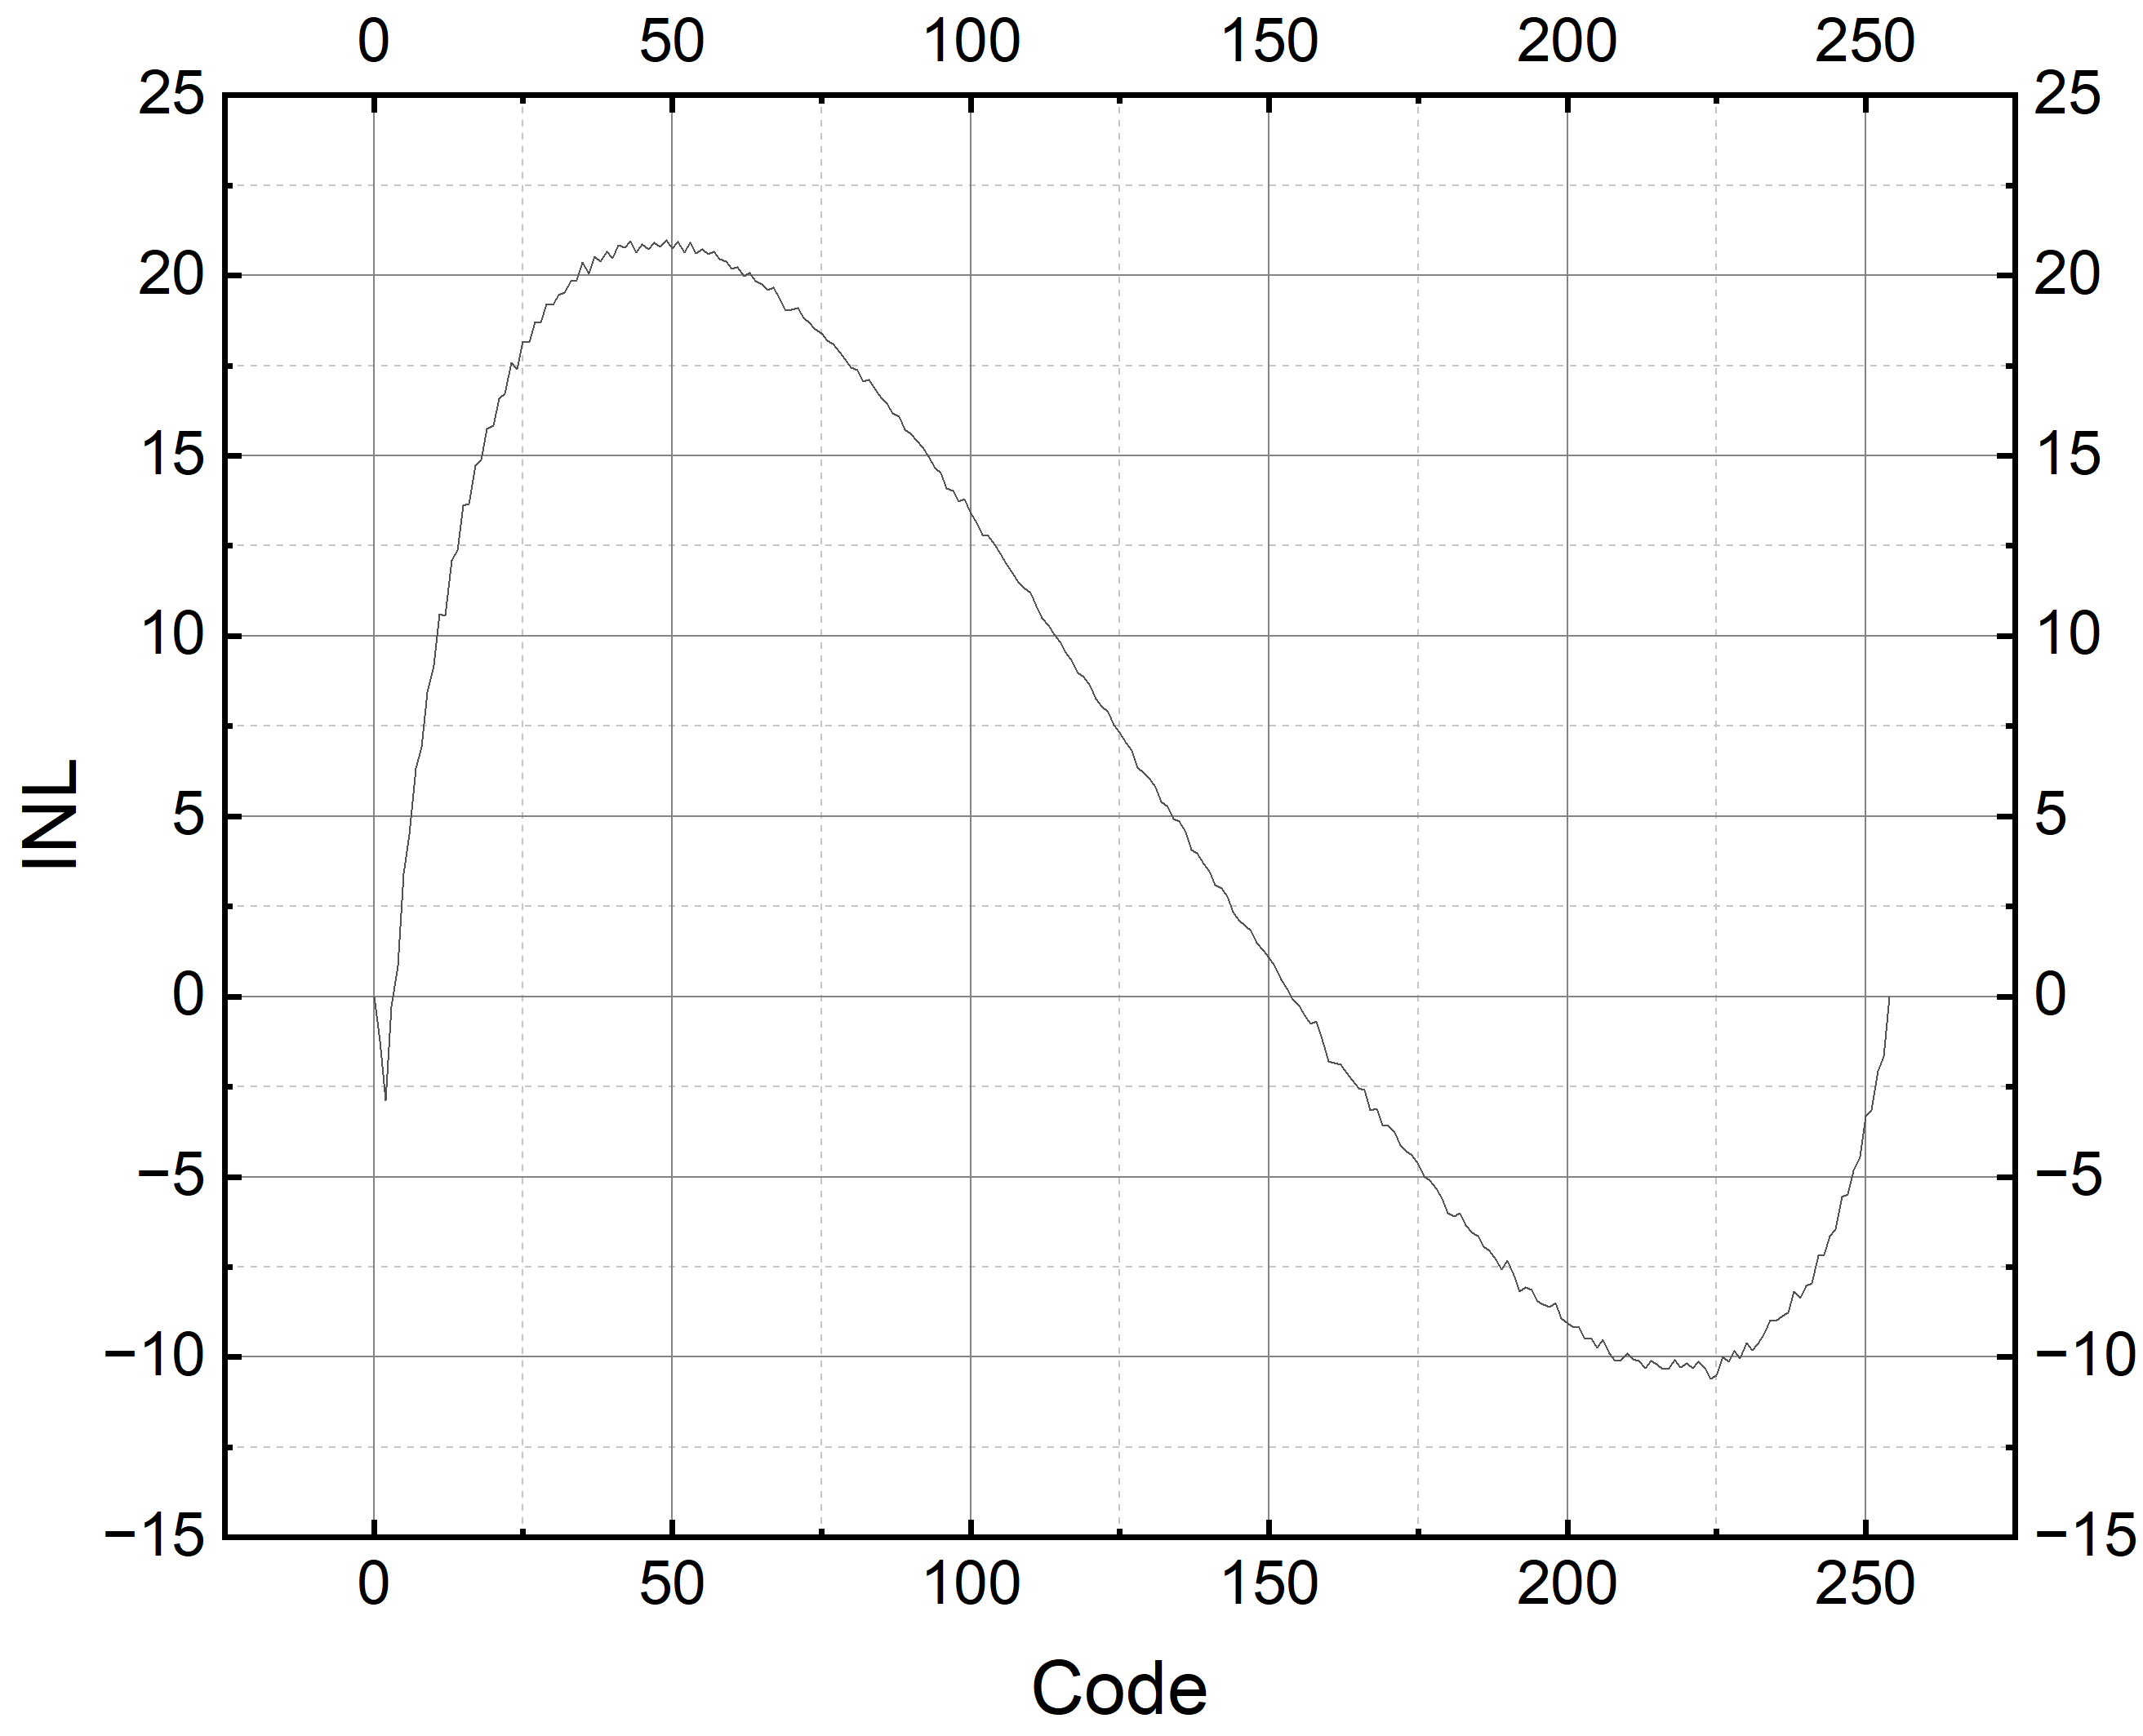
\includegraphics[width=\linewidth]{figures/Results/Previous Implementation-INL.png}
    \caption{\gls{inl} of the \gls{csi}-\gls{dac} delay line.}
    \label{fig:current_starved_dac_inl}
  \end{subfigure}
  \hfill
  \begin{subfigure}{0.4\linewidth}
    \centering
    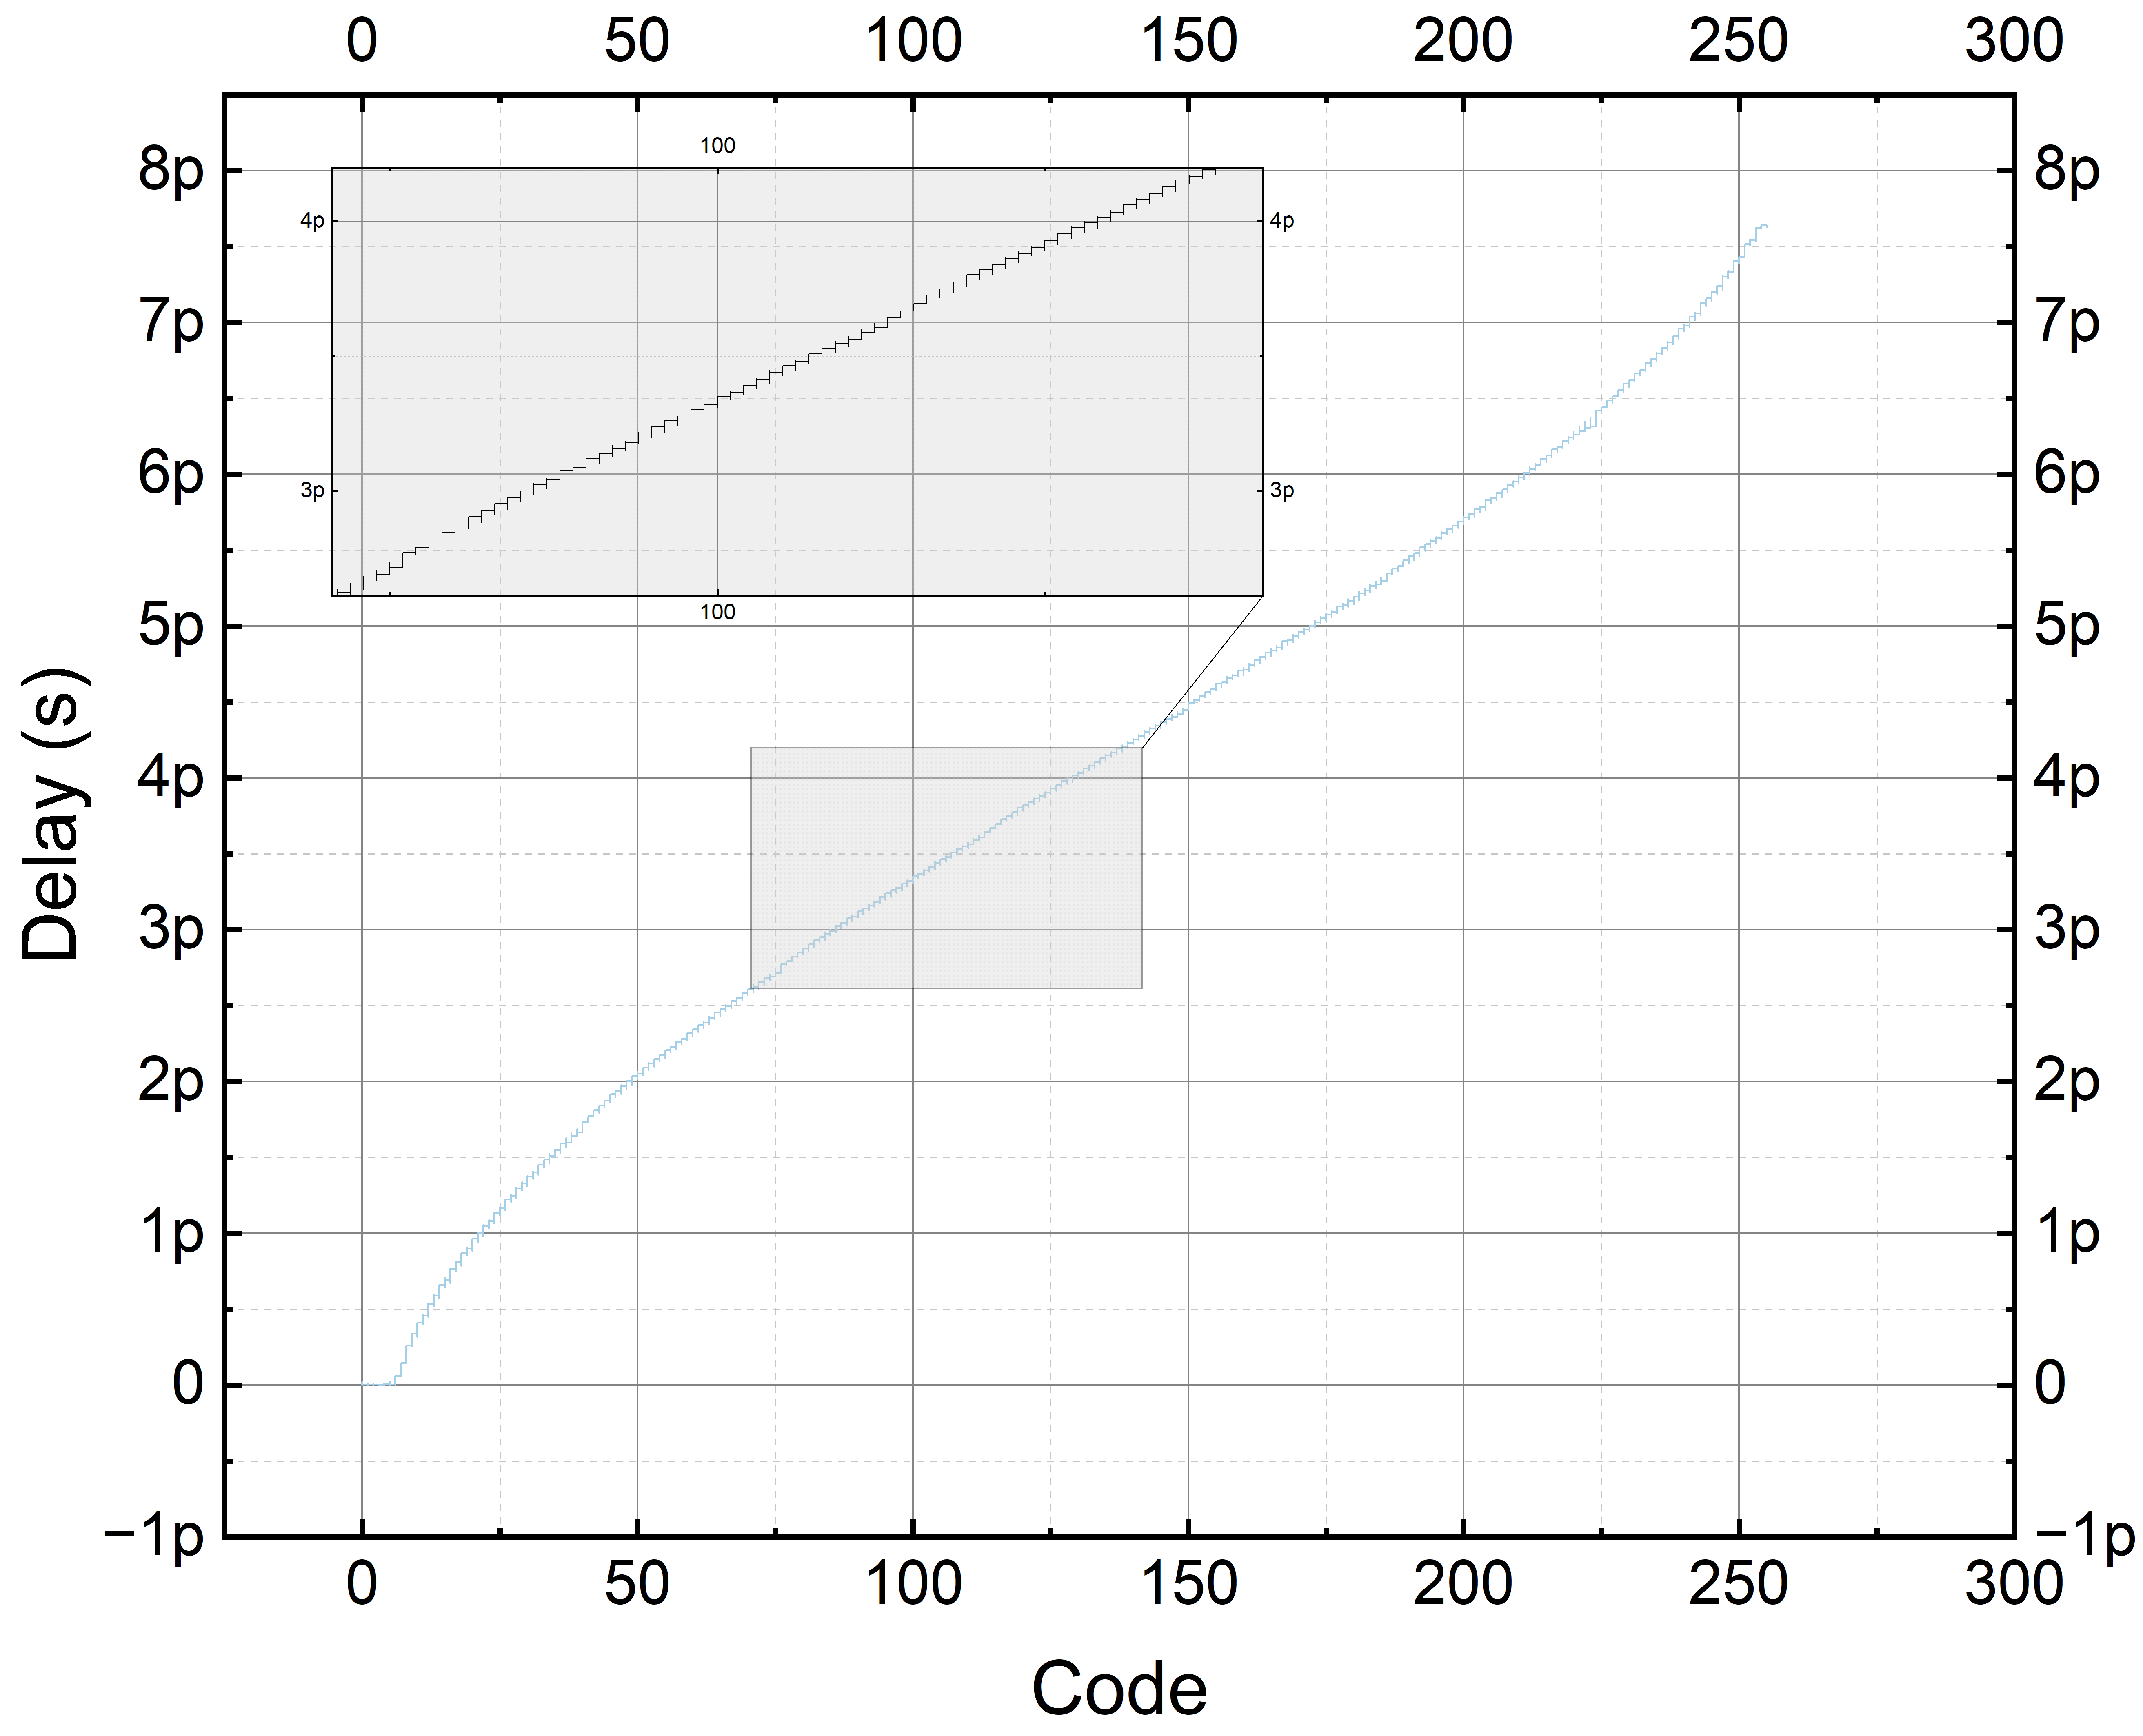
\includegraphics[width=\linewidth]{figures/Results/Previous Implementation-DelayAcrossCodesWithZoomIN.png}
    \caption{Delay across codes of the previous \gls{csi}-\gls{dac} delay line.}
    \label{fig:current_starved_dac_delay_range}
  \end{subfigure}
  \caption{Characteristics of the previous current-starved delay stage implementation.}
\end{figure}

\begin{figure}[htbp]
  \centering
  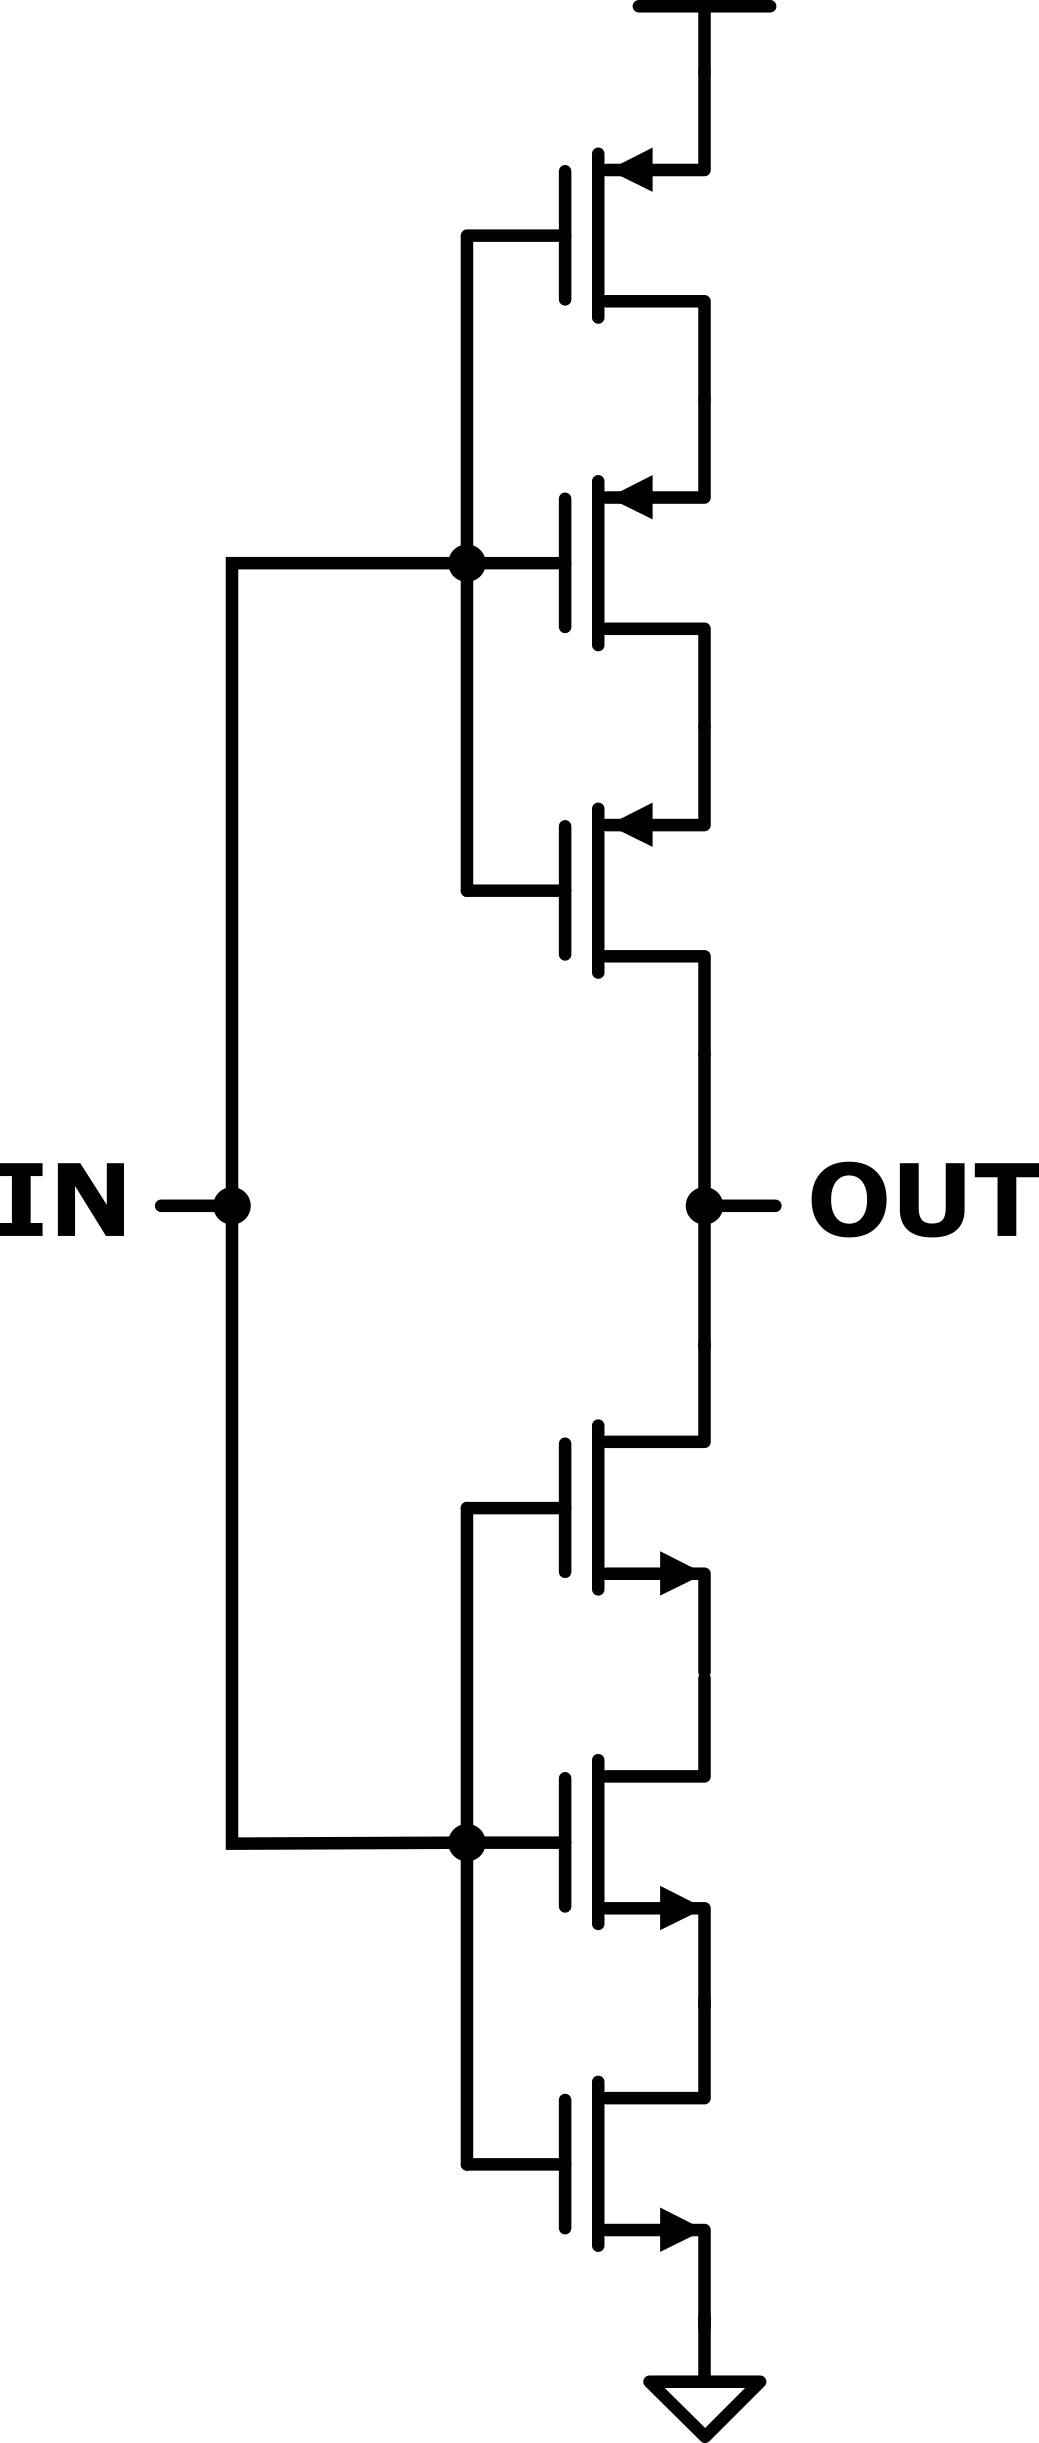
\includegraphics[width=0.3\linewidth, angle=90]{figures/Schematics/stacked_inverter-2.png}
  \caption{Stacked MOS inverter topology for edge balancing.}
  \label{fig:stacked_inv}
\end{figure}

\begin{figure}[htbp]
  \centering
  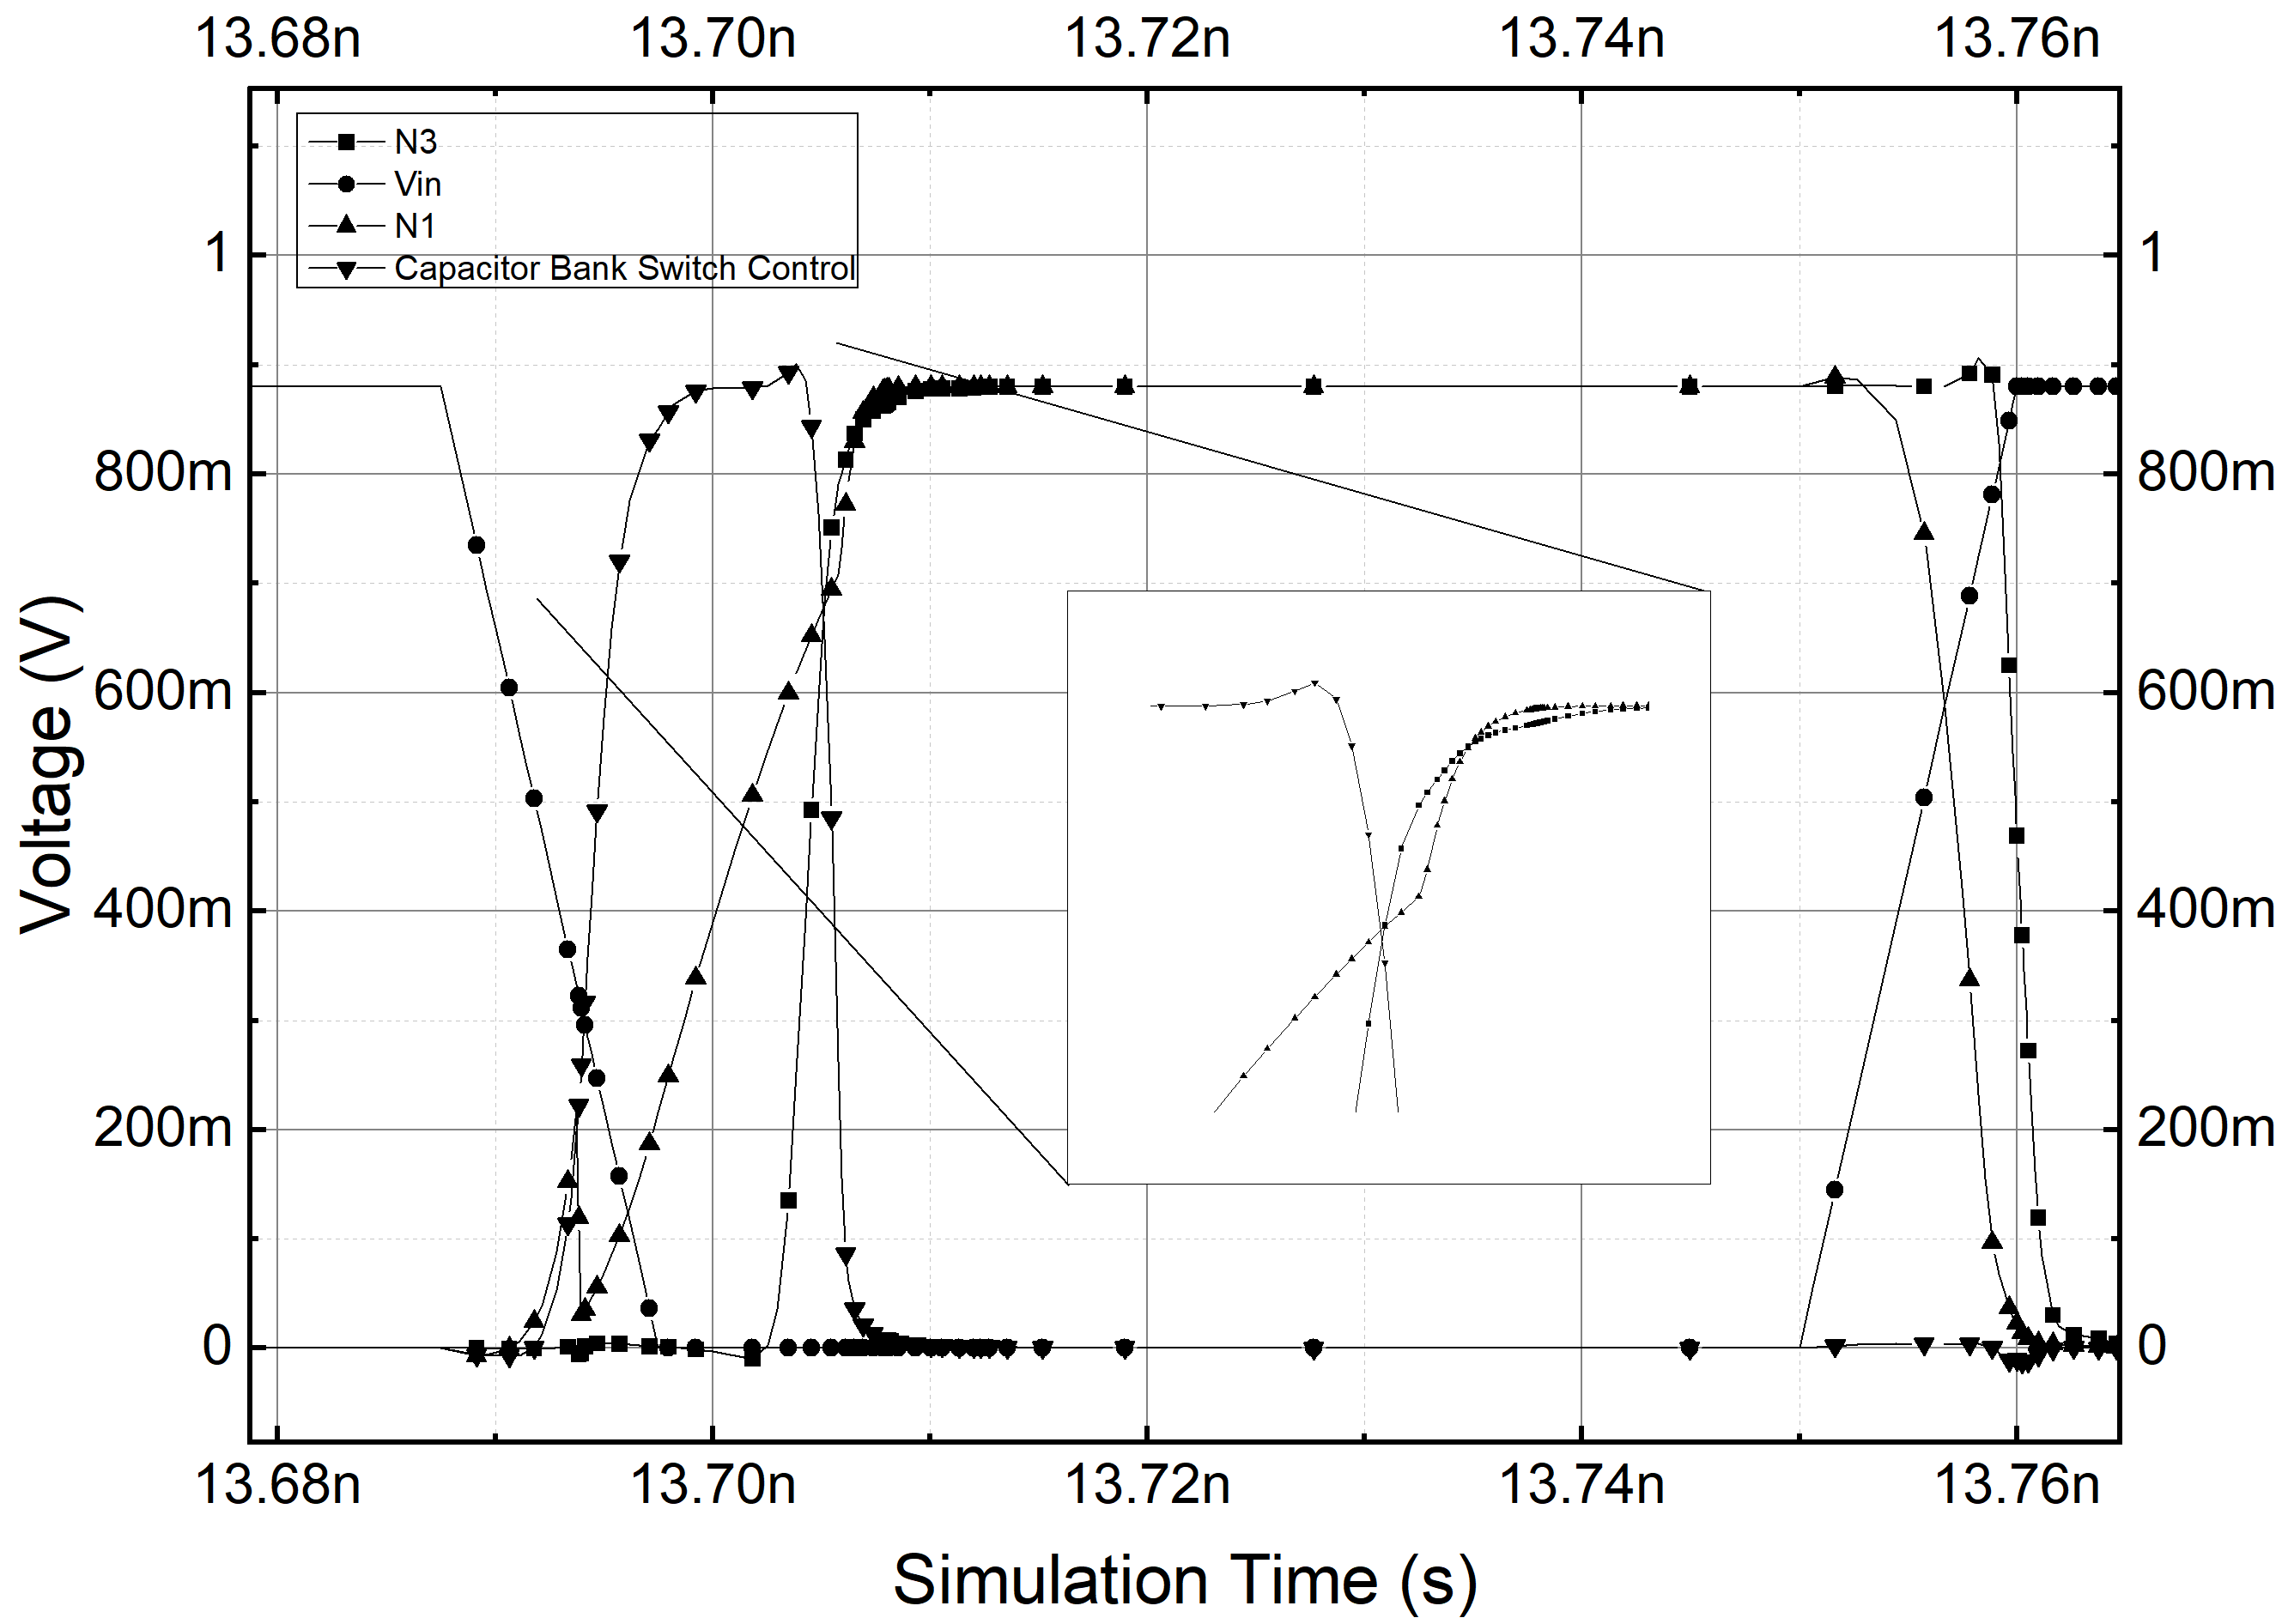
\includegraphics[width=0.5\linewidth]{figures/Results/SCI-SwitchVoltageAndLoadingTime.png}
  \caption{Switched capacitor tap switch closing and charging the capacitor to Node~1. A zoomed view of the voltage at Node~1 shows two distinct rise rates.}
  \label{fig:switched_cap_charging_cap_switch}
\end{figure}

\begin{figure}[htbp]
  \centering
  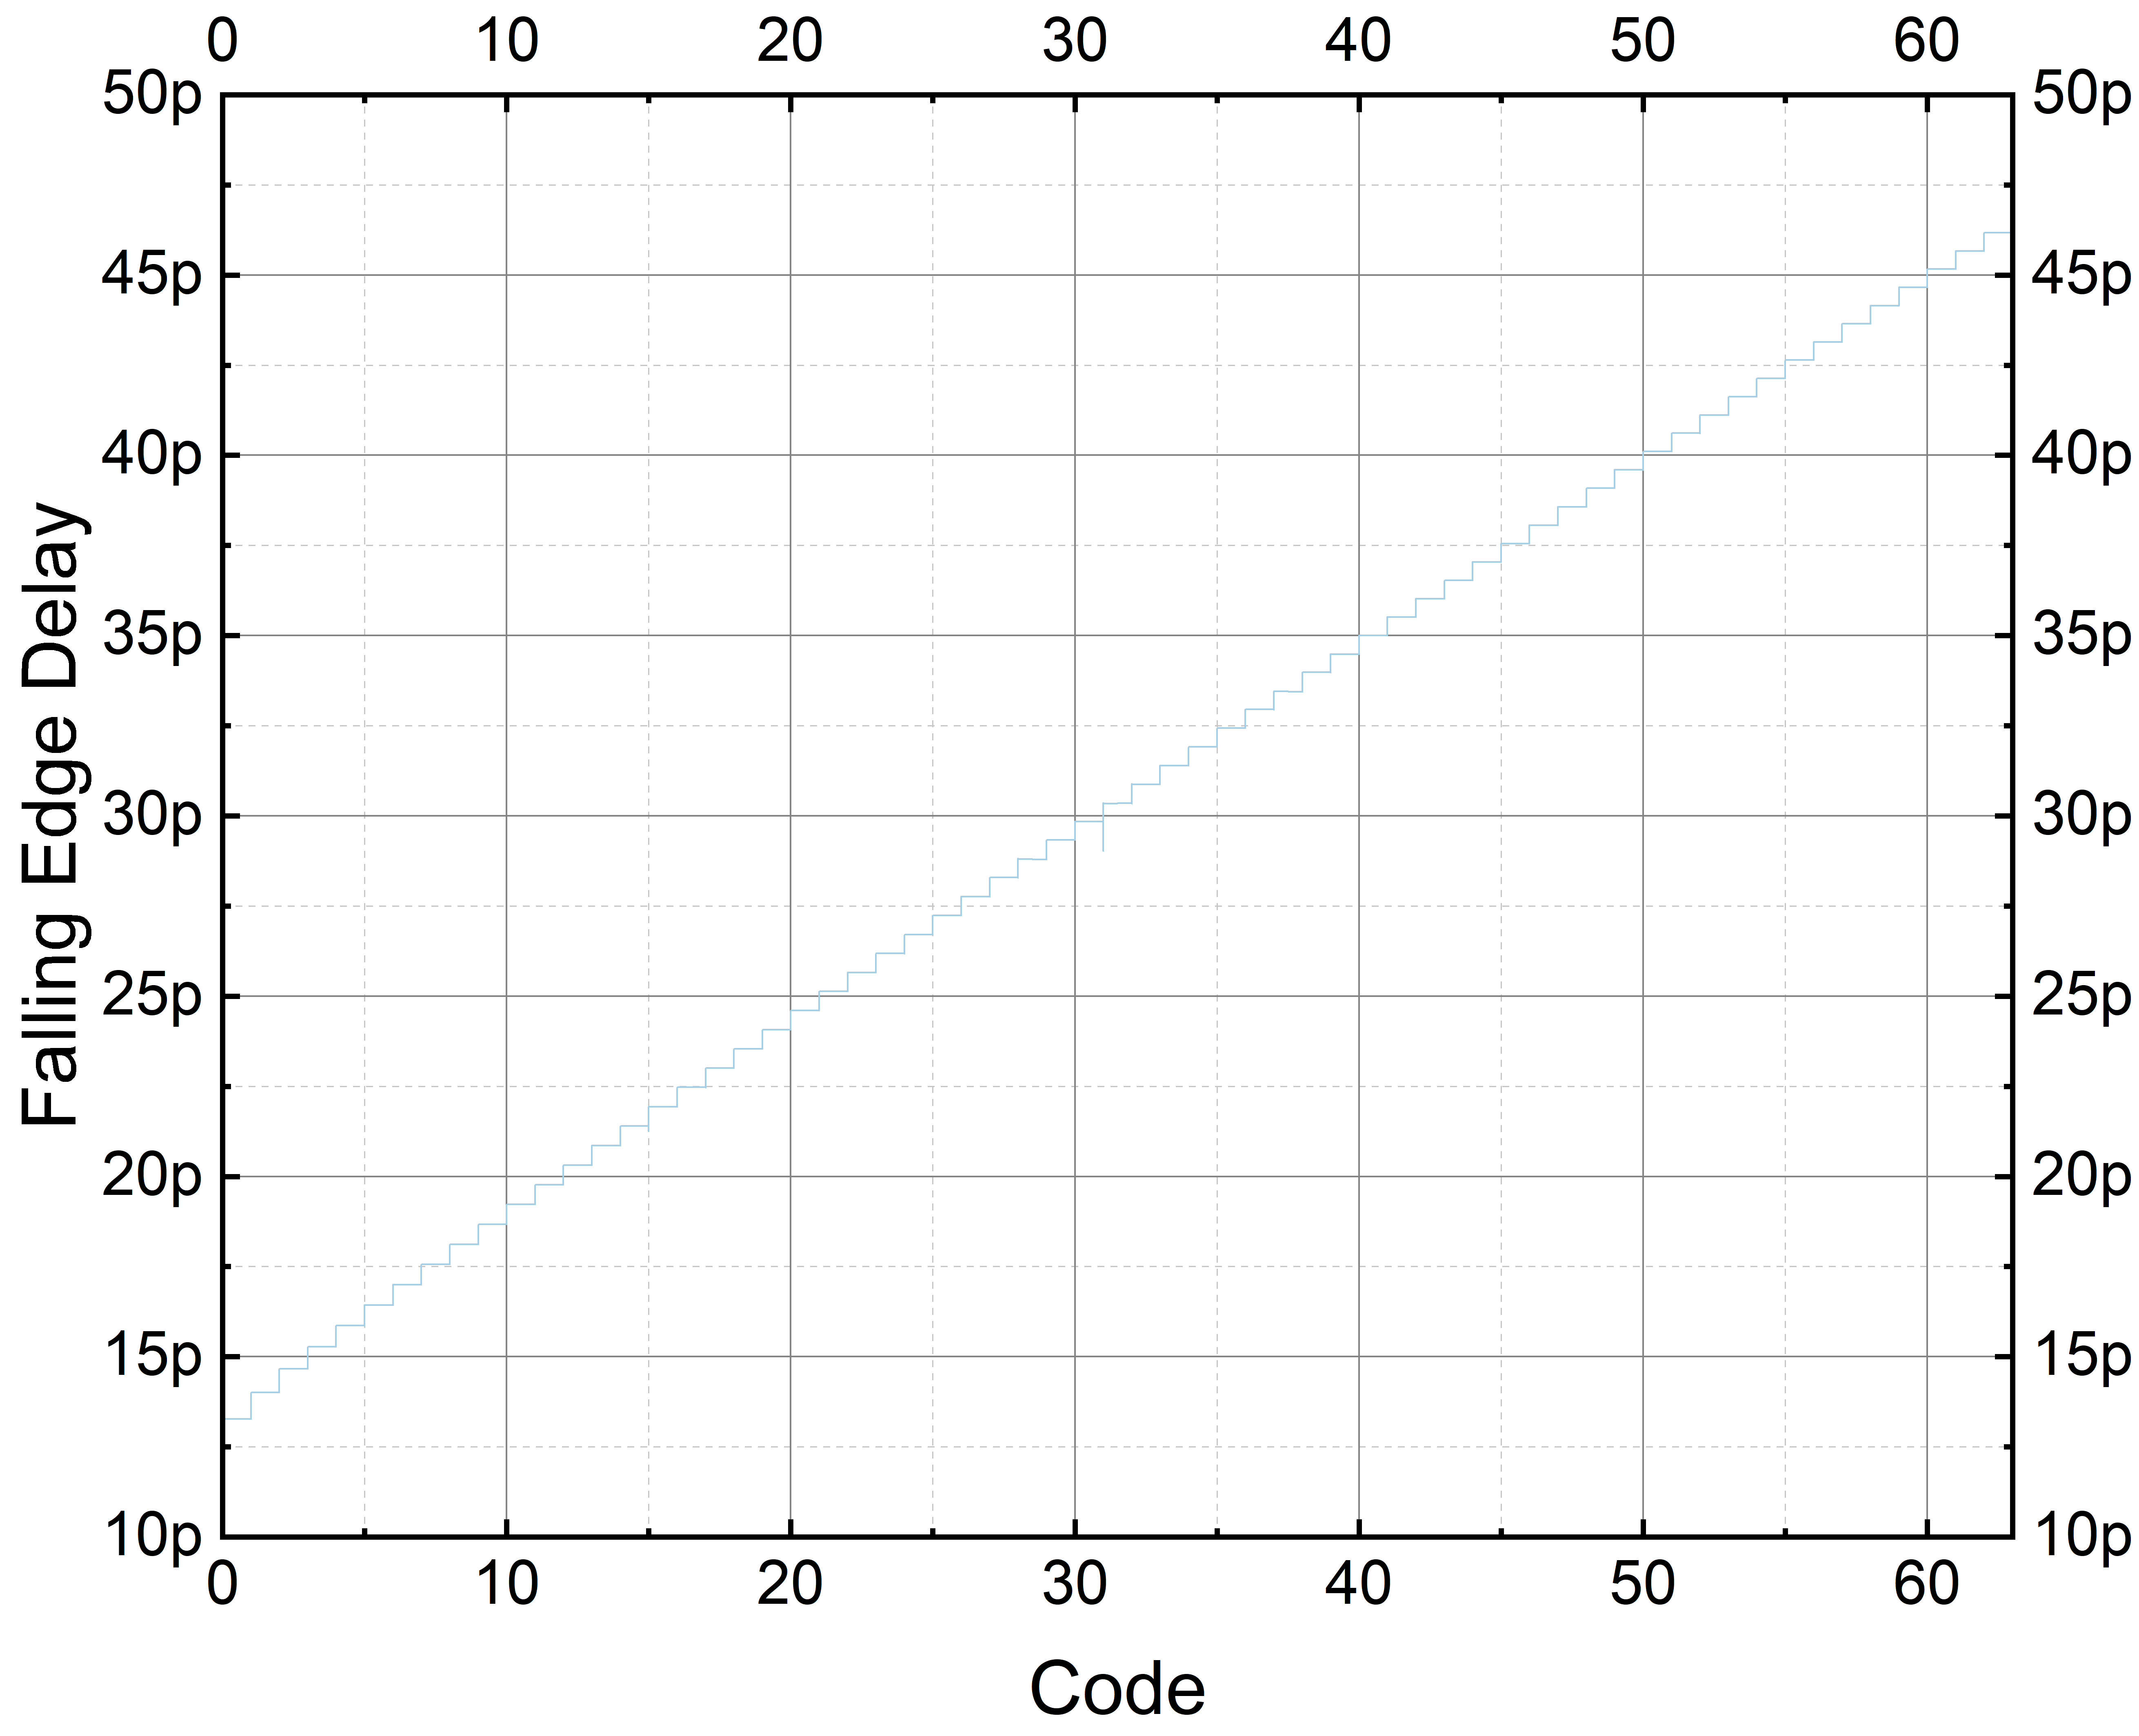
\includegraphics[width=0.5\linewidth]{figures/Results/SCI-FallingEdgeDelay.png}
  \caption{Delay across codes of the switched capacitor delay element. Codes switched across time.}
  \label{fig:SCI_delayacrosscodes}
\end{figure}

\begin{figure}[htbp]
  \centering
  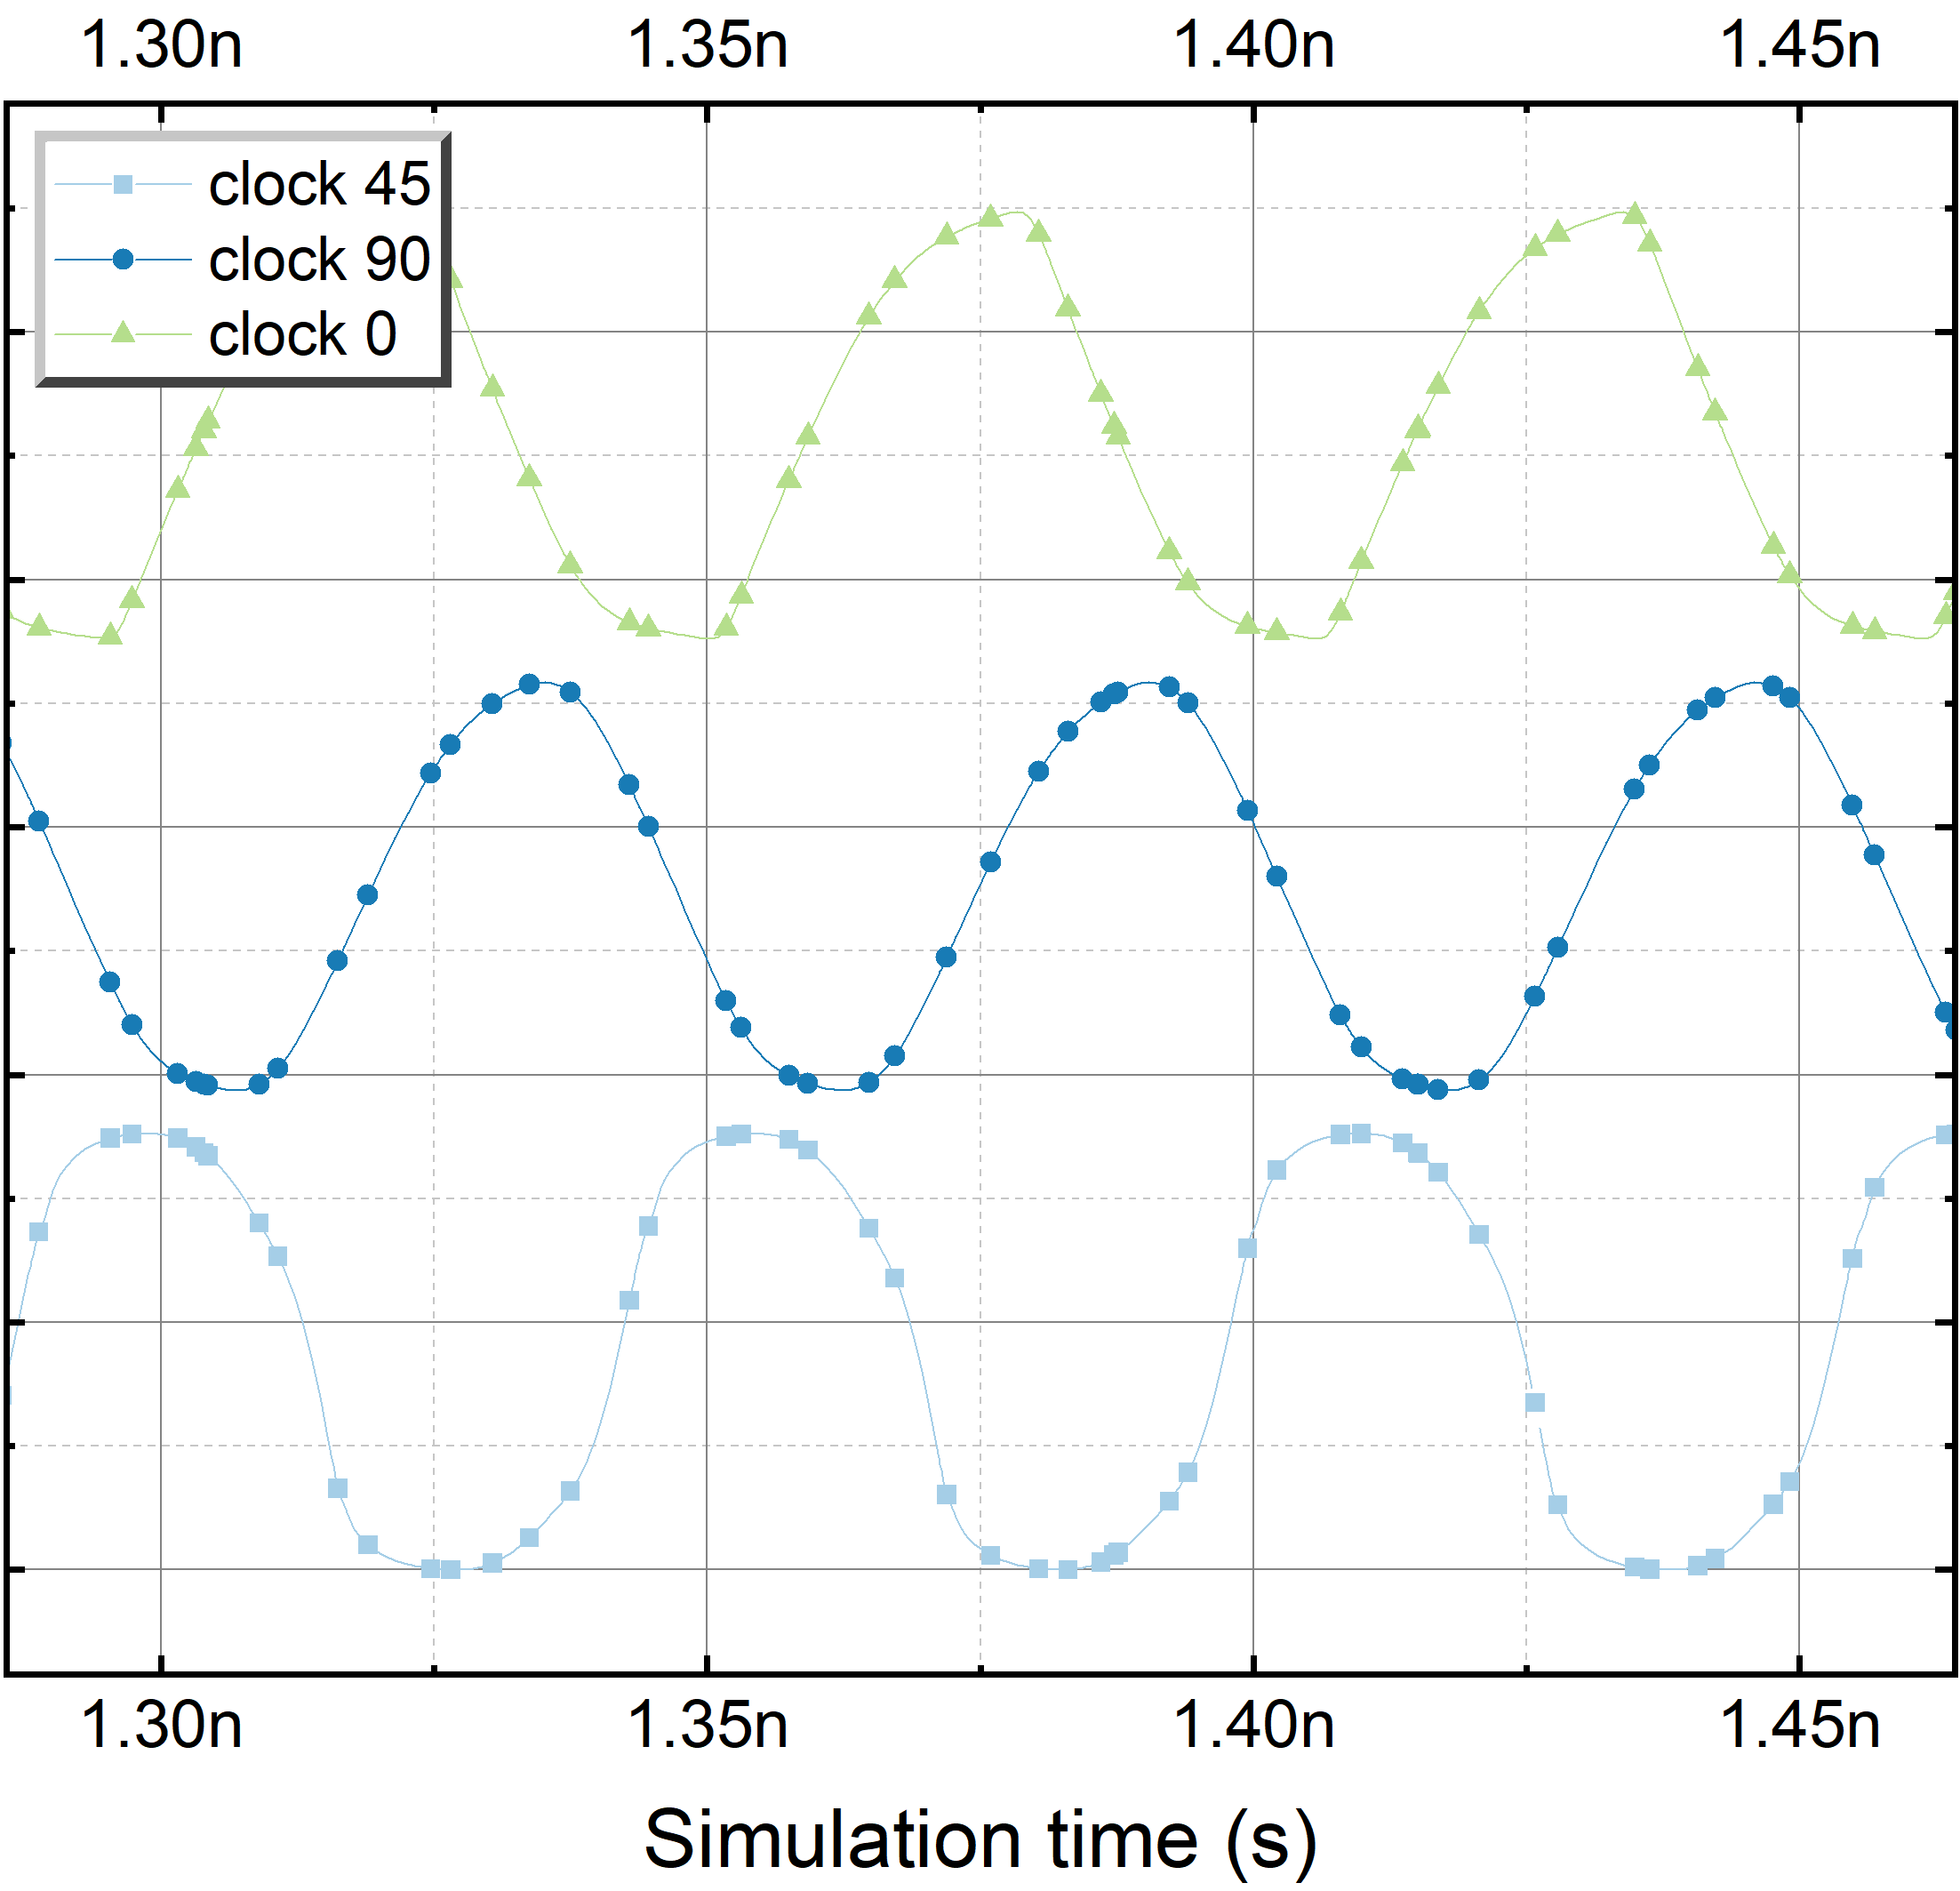
\includegraphics[width=0.5\linewidth]{figures/Results/PI_8out_CSI-clock0Clock90MixingBuildingClock45.png}
  \caption{Mixing waveforms from the fast (\ang{45}) and slow (\ang{90}) paths. The mixed waveform is the result of the two paths converging at the mixing node, \ang{45}.}
  \label{fig:PI_1_mixing_waveforms}
\end{figure}

\begin{figure}[htbp]
  \centering
  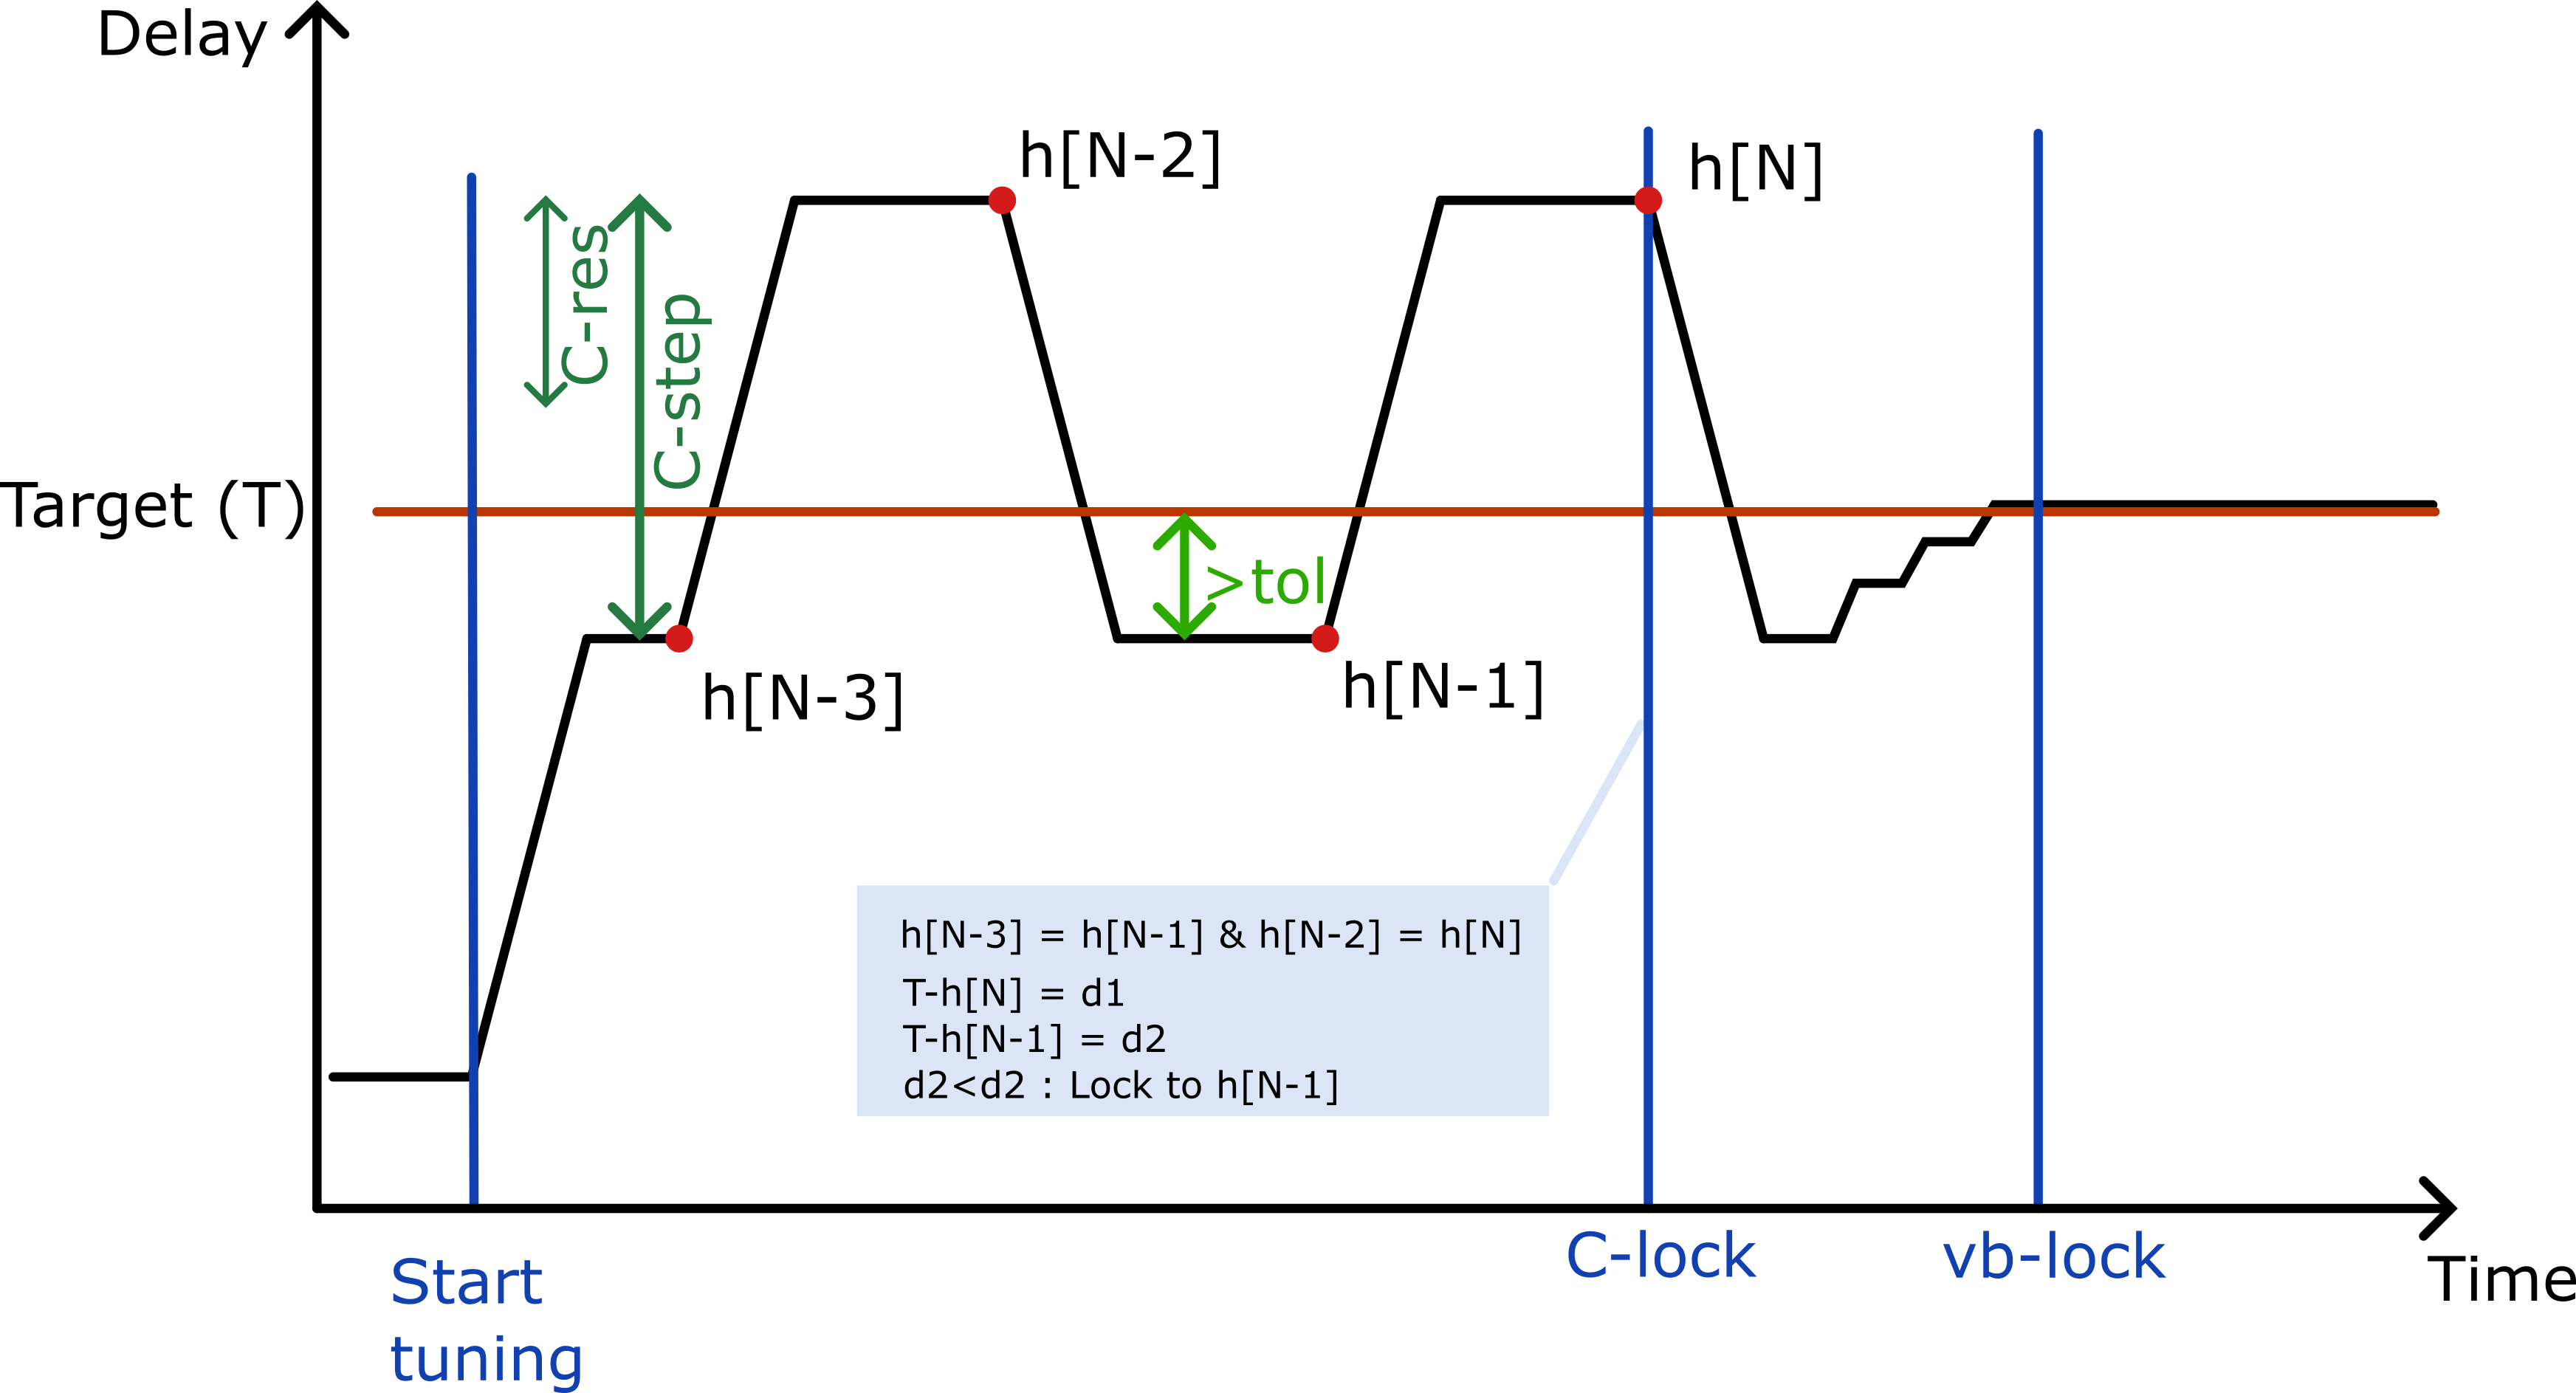
\includegraphics[width=0.8\textwidth]{figures/Schematics/Tuning_principle.png}
  \caption{Visual representation of the tuning mechanism. In this example, the coarse tuner never reaches close enough to the target phase, so it oscillates. The Verilog-A block detects this, compares history samples and locks at the best phase. The fine tuner then takes over and adjusts the phase to the target value.}
  \label{fig:tuning_hierarchy}
\end{figure}

\begin{figure}[htbp]
  \centering
  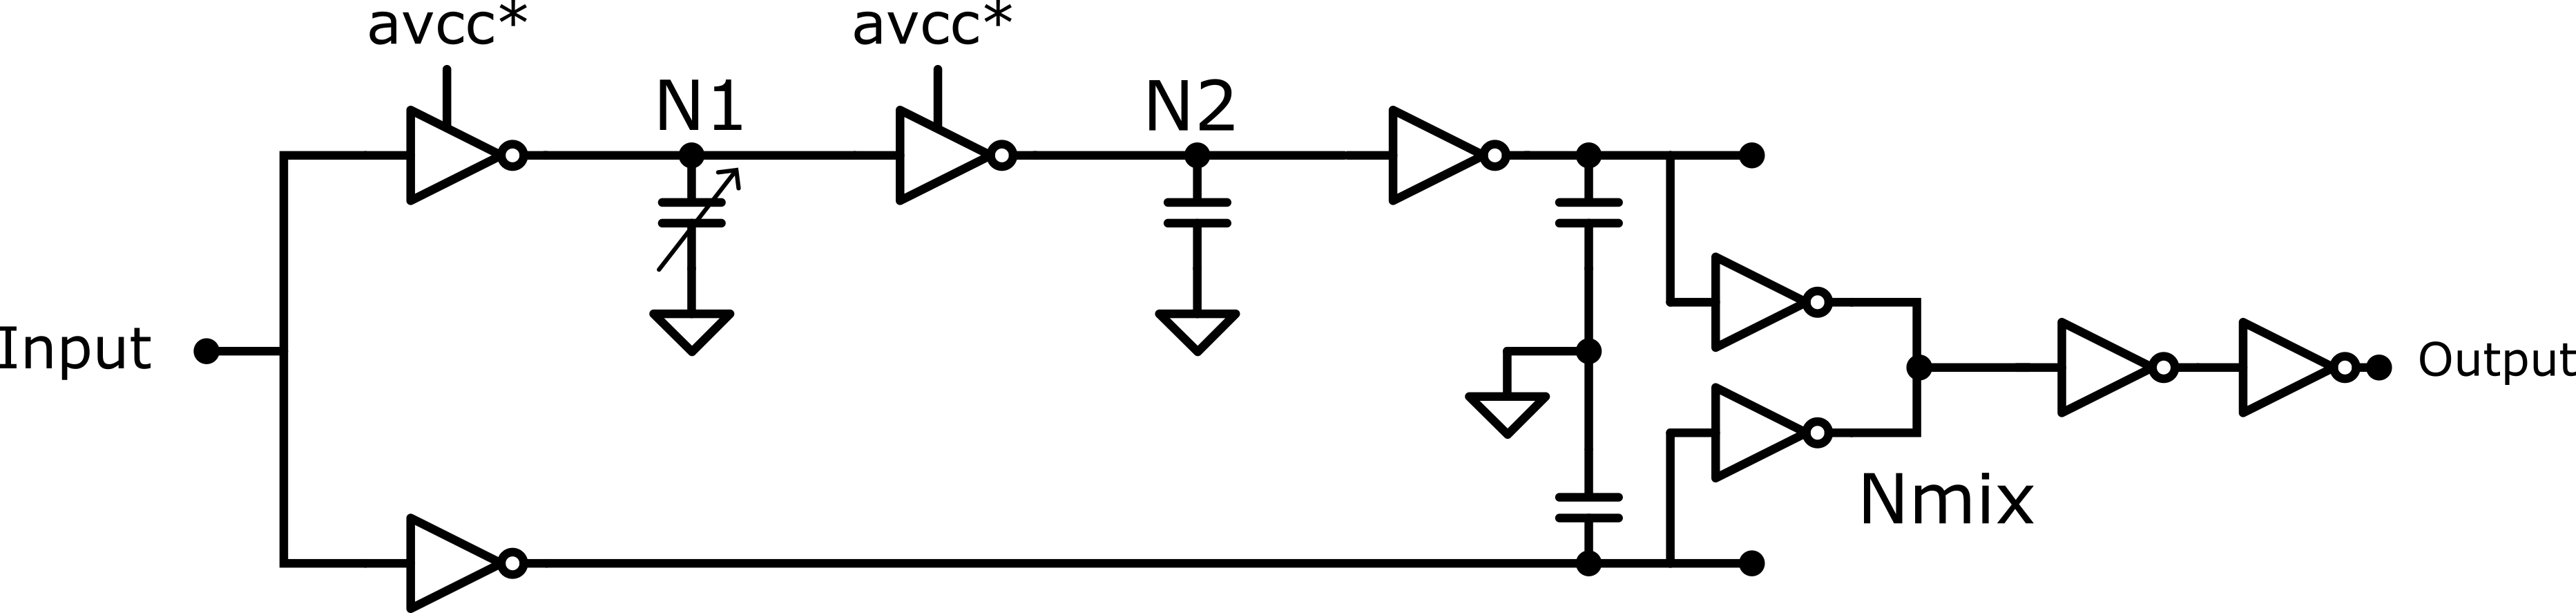
\includegraphics[width=0.8\linewidth]{figures/Schematics/clock_generation_half_V2.png}
  \caption{Phase interpolator with two-stage supply-bias fine-tuning.}
  \label{fig:PI_2_schematic}
\end{figure}

\begin{figure}[htbp]
  \centering
  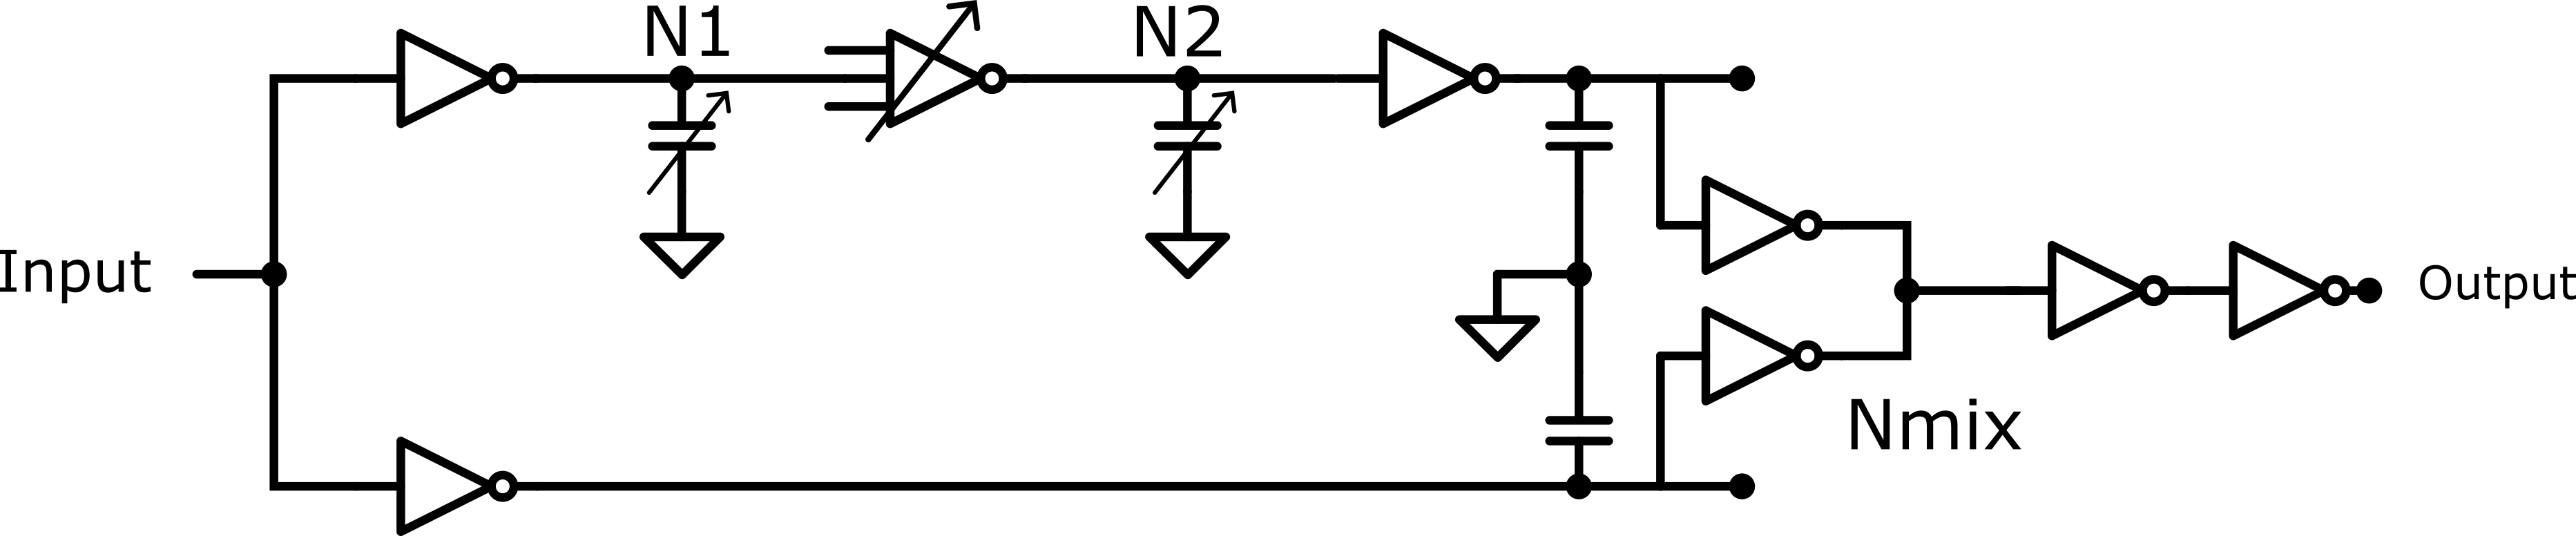
\includegraphics[width=0.8\linewidth]{figures/Schematics/clock_generation_half_CSI.png}
  \caption{Phase interpolator with current-starved inverter fine-tuning.}
  \label{fig:PI_csi_schematic}
\end{figure}

\begin{figure}[htbp]
  \centering
  \begin{subfigure}[b]{0.40\linewidth}
    \centering
    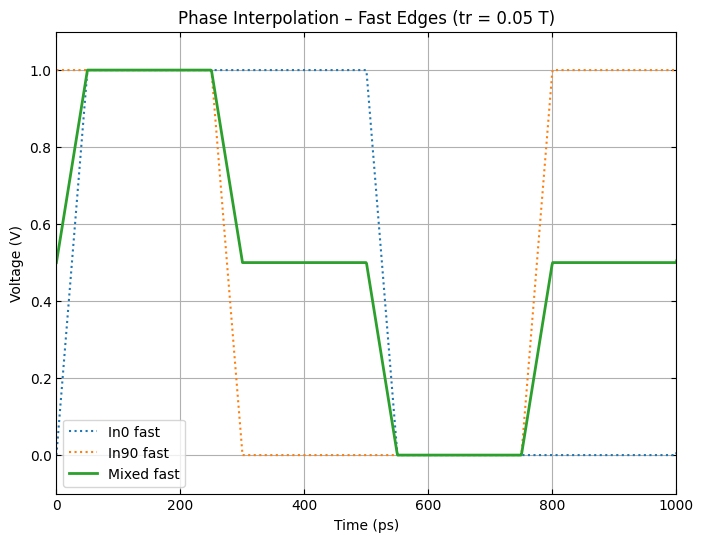
\includegraphics[width=\linewidth]{figures/Python/pi_fast_edges.png}
    \caption{Fast edges, $t_{\text{rise}}\!\ll\!1/(4f)$}
    \label{fig:fast}
  \end{subfigure}
  \hfill
  \begin{subfigure}[b]{0.40\linewidth}
    \centering
    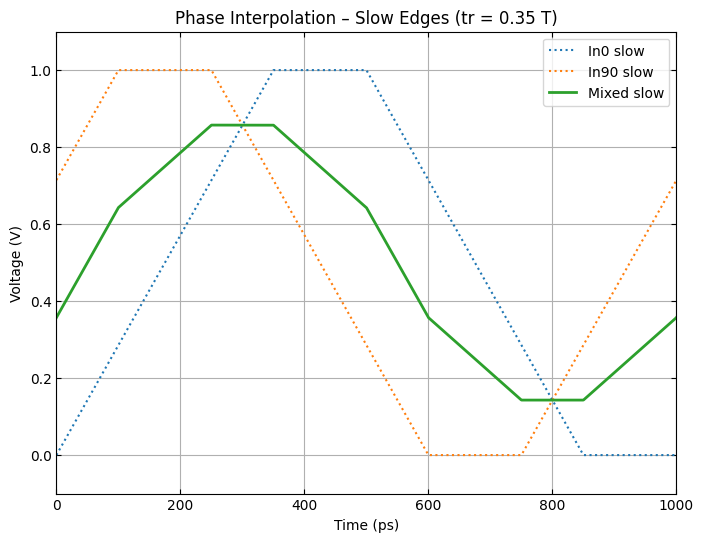
\includegraphics[width=\linewidth]{figures/Python/pi_slow_edges.png}
    \caption{Slow edges satisfying~(\ref{eq:overlap})}
    \label{fig:slow}
  \end{subfigure}
  \caption{Phase‑interpolator input edges and the resulting mid‑rail behaviour.}
  \label{fig:pi_edges}
\end{figure}

\begin{figure}[htbp]
  \centering
  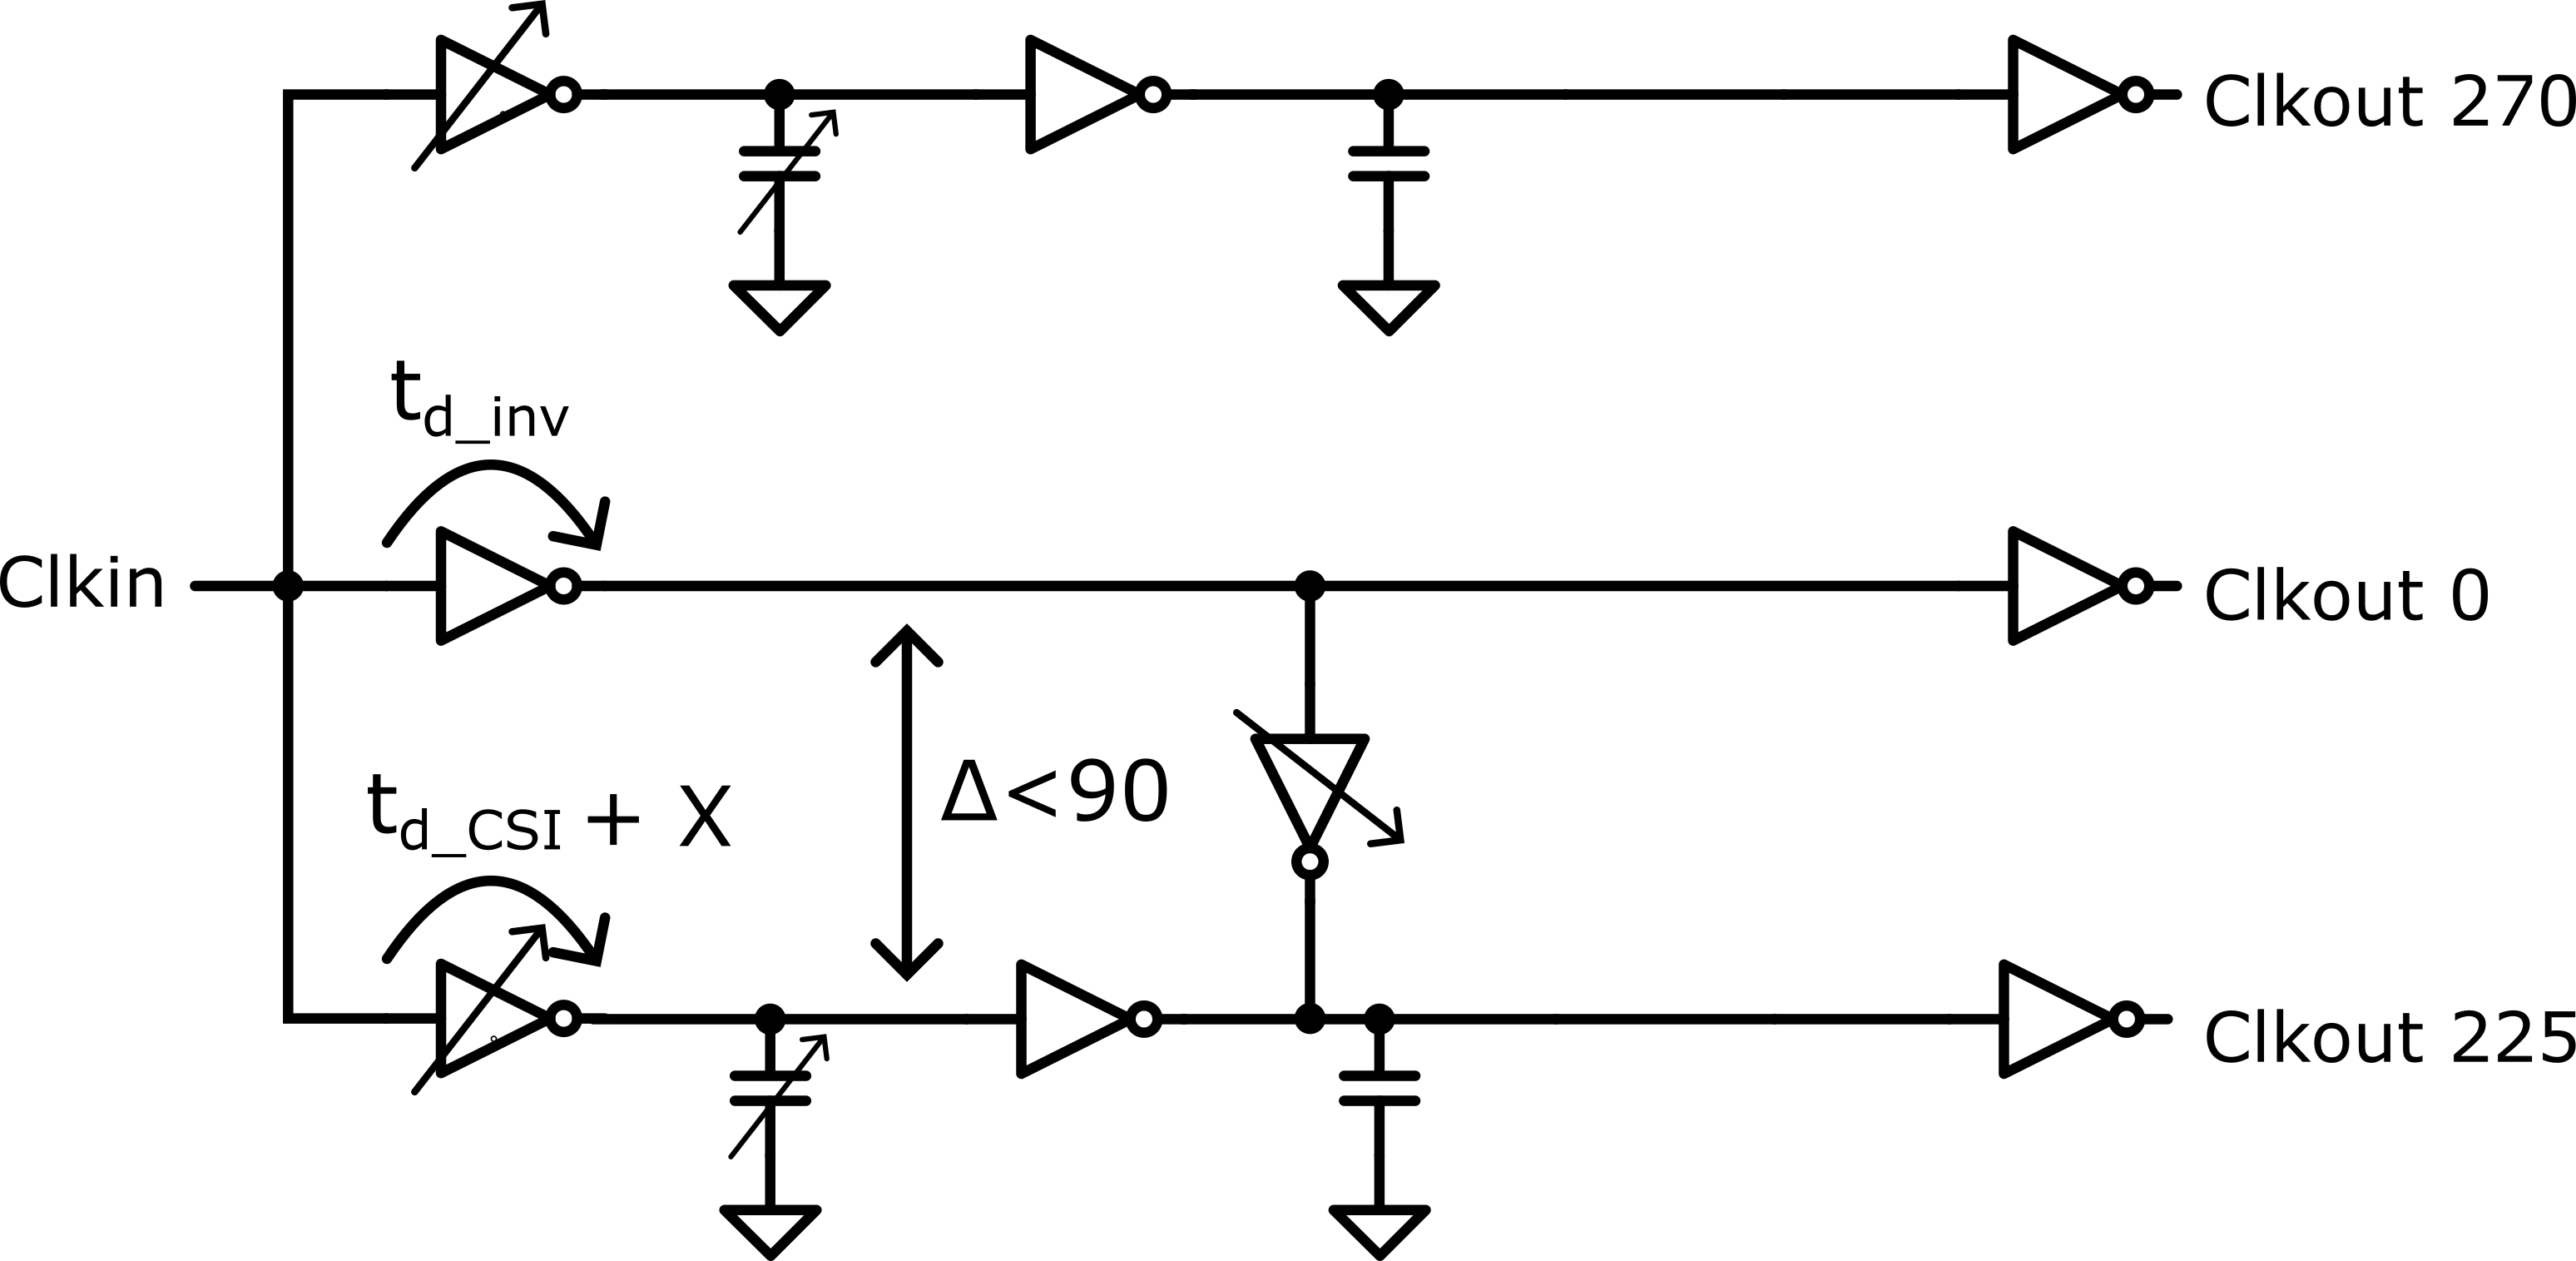
\includegraphics[width=0.6\linewidth]{figures/Schematics/ff_csi_3out.png}
  \caption{Feed-forward phase interpolator with internal node with phase $\approx$\ang{180} feeding into a second intermediate node with delay $\approx$\ang{135}.}
  \label{fig:FF_half_1}
\end{figure}

\begin{figure}[htbp]
  \centering
  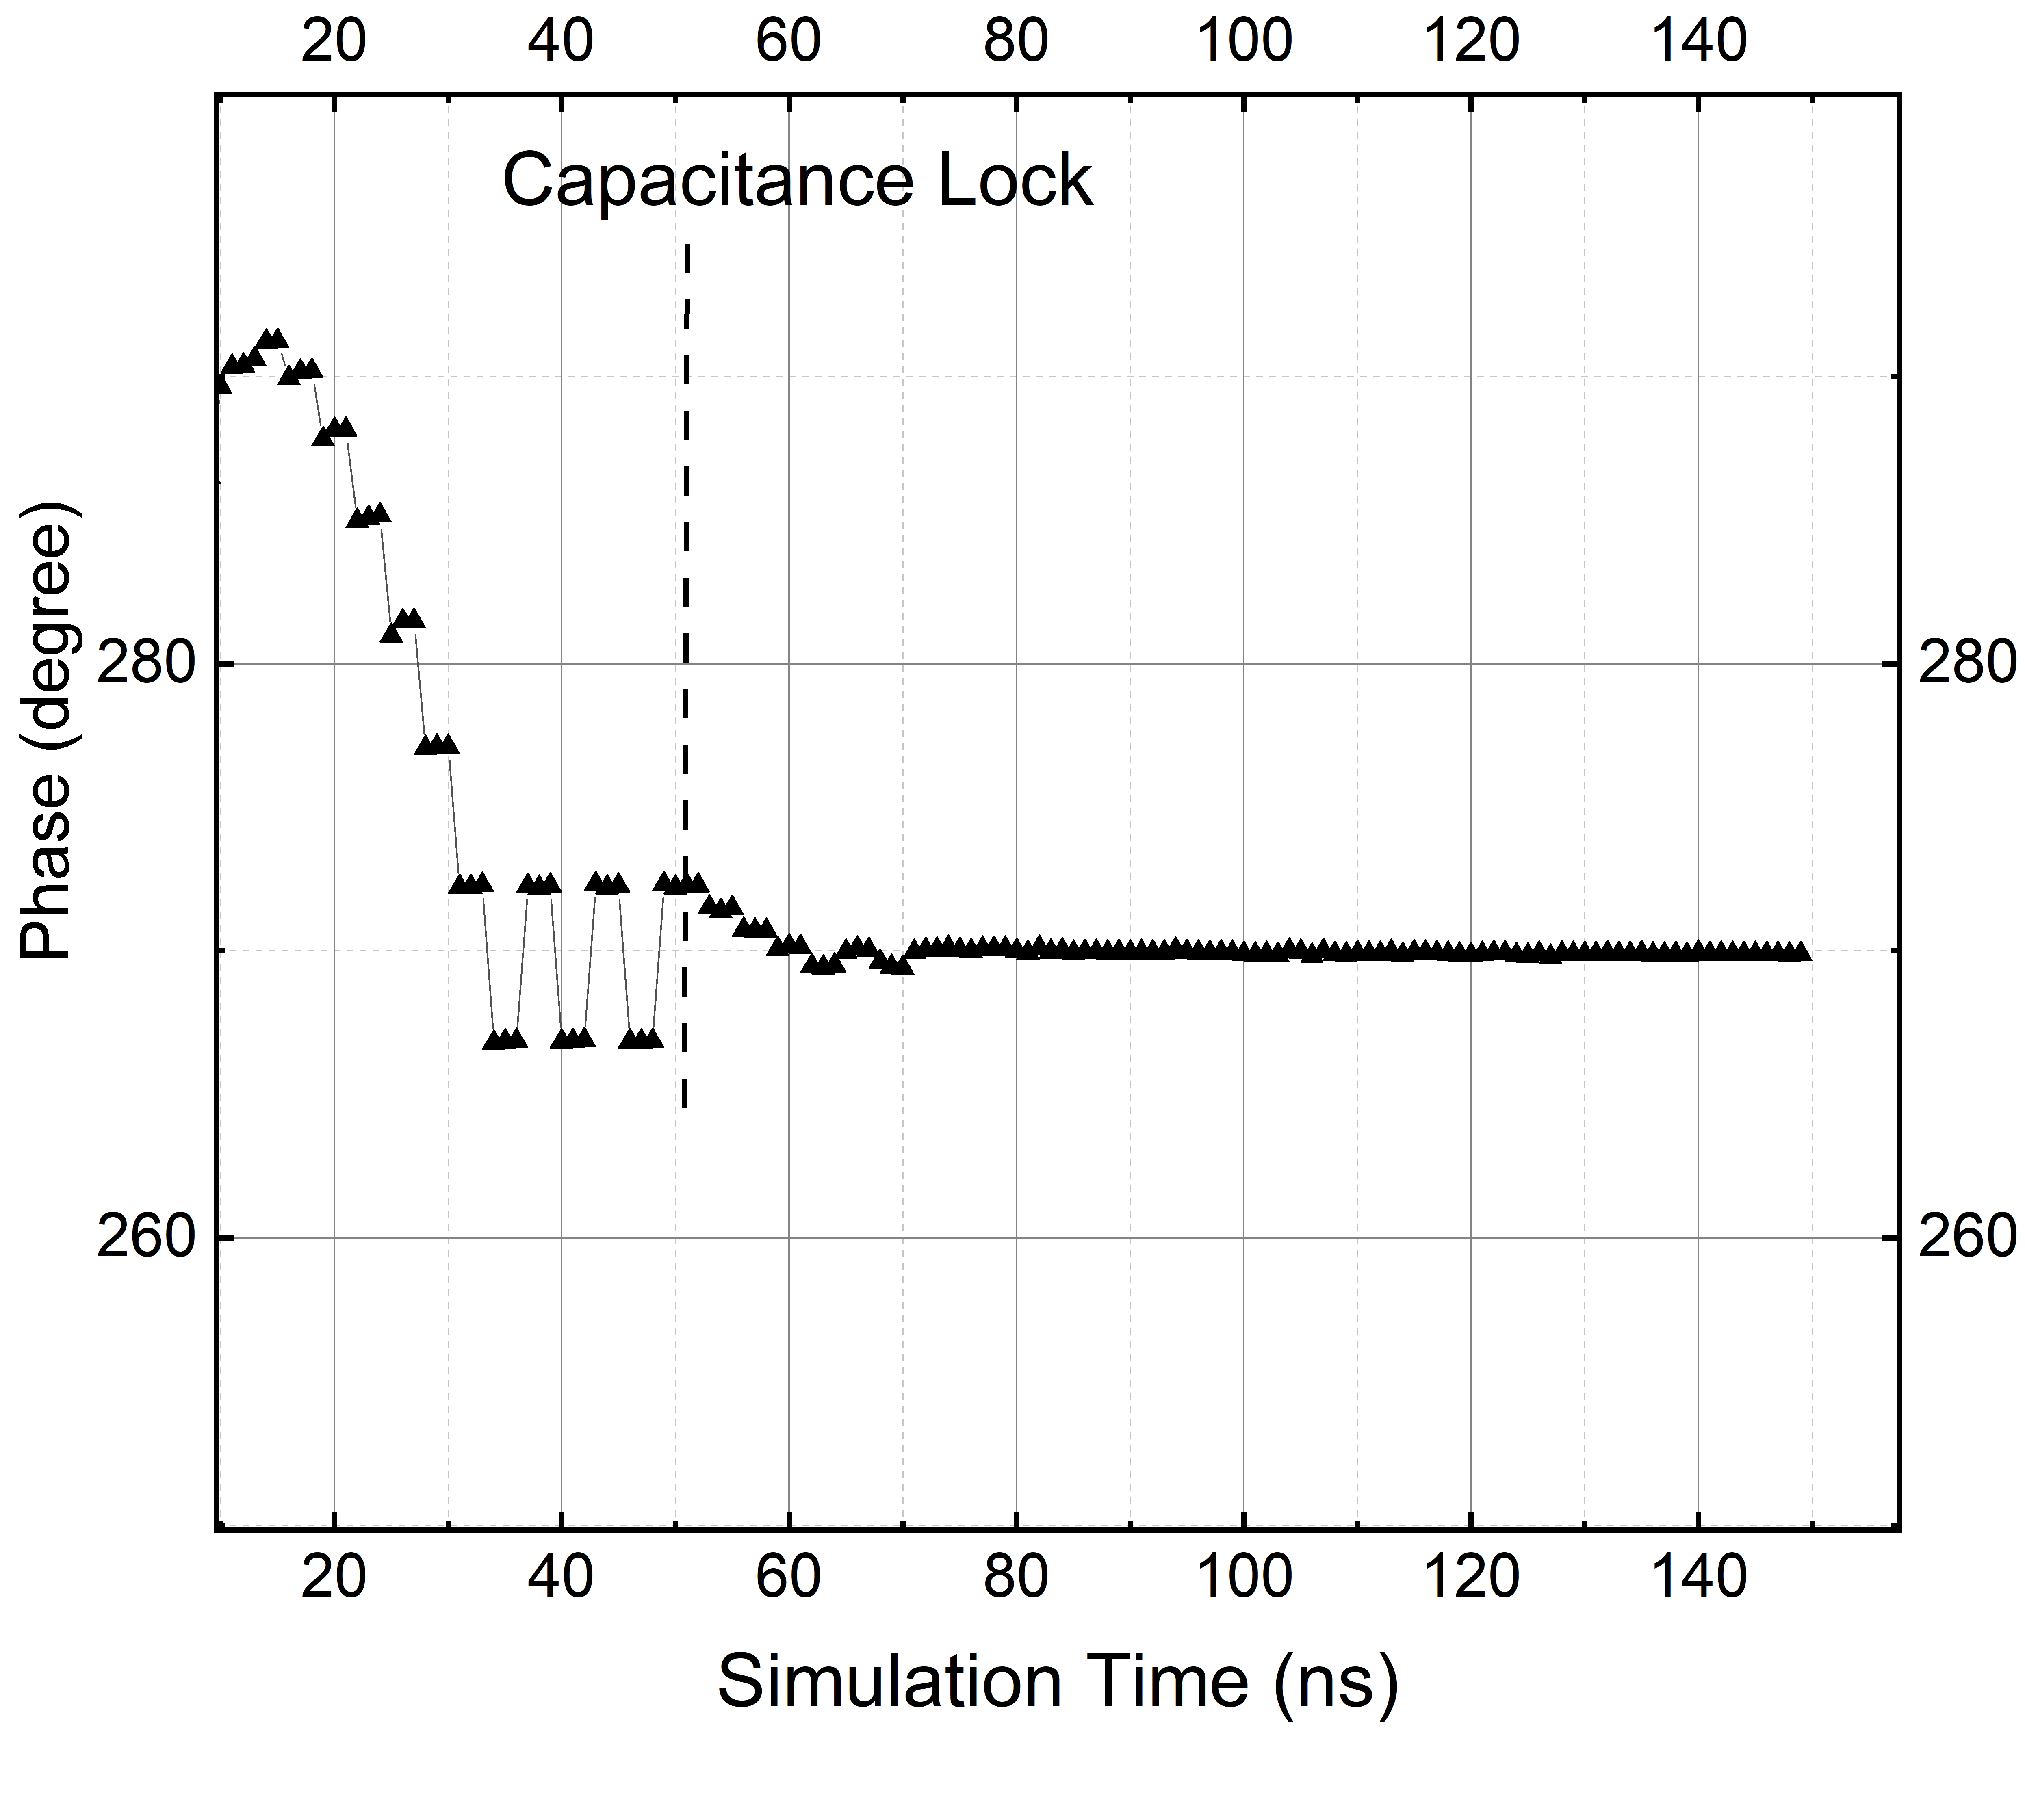
\includegraphics[width=0.5\linewidth]{figures/Results/FF_3out_CSI_dynamicTuning-225And270TuningCapAndVb.png}
  \caption{Verilog-A tuning of the feed-forward phase interpolator. The coarse steps are followed by fine-tuning the bias voltages of the current-starved inverter (\gls{csi}).}
  \label{fig:FF_half_Verilog-A_tuning}
\end{figure}

\begin{figure}[htbp]
  \centering
  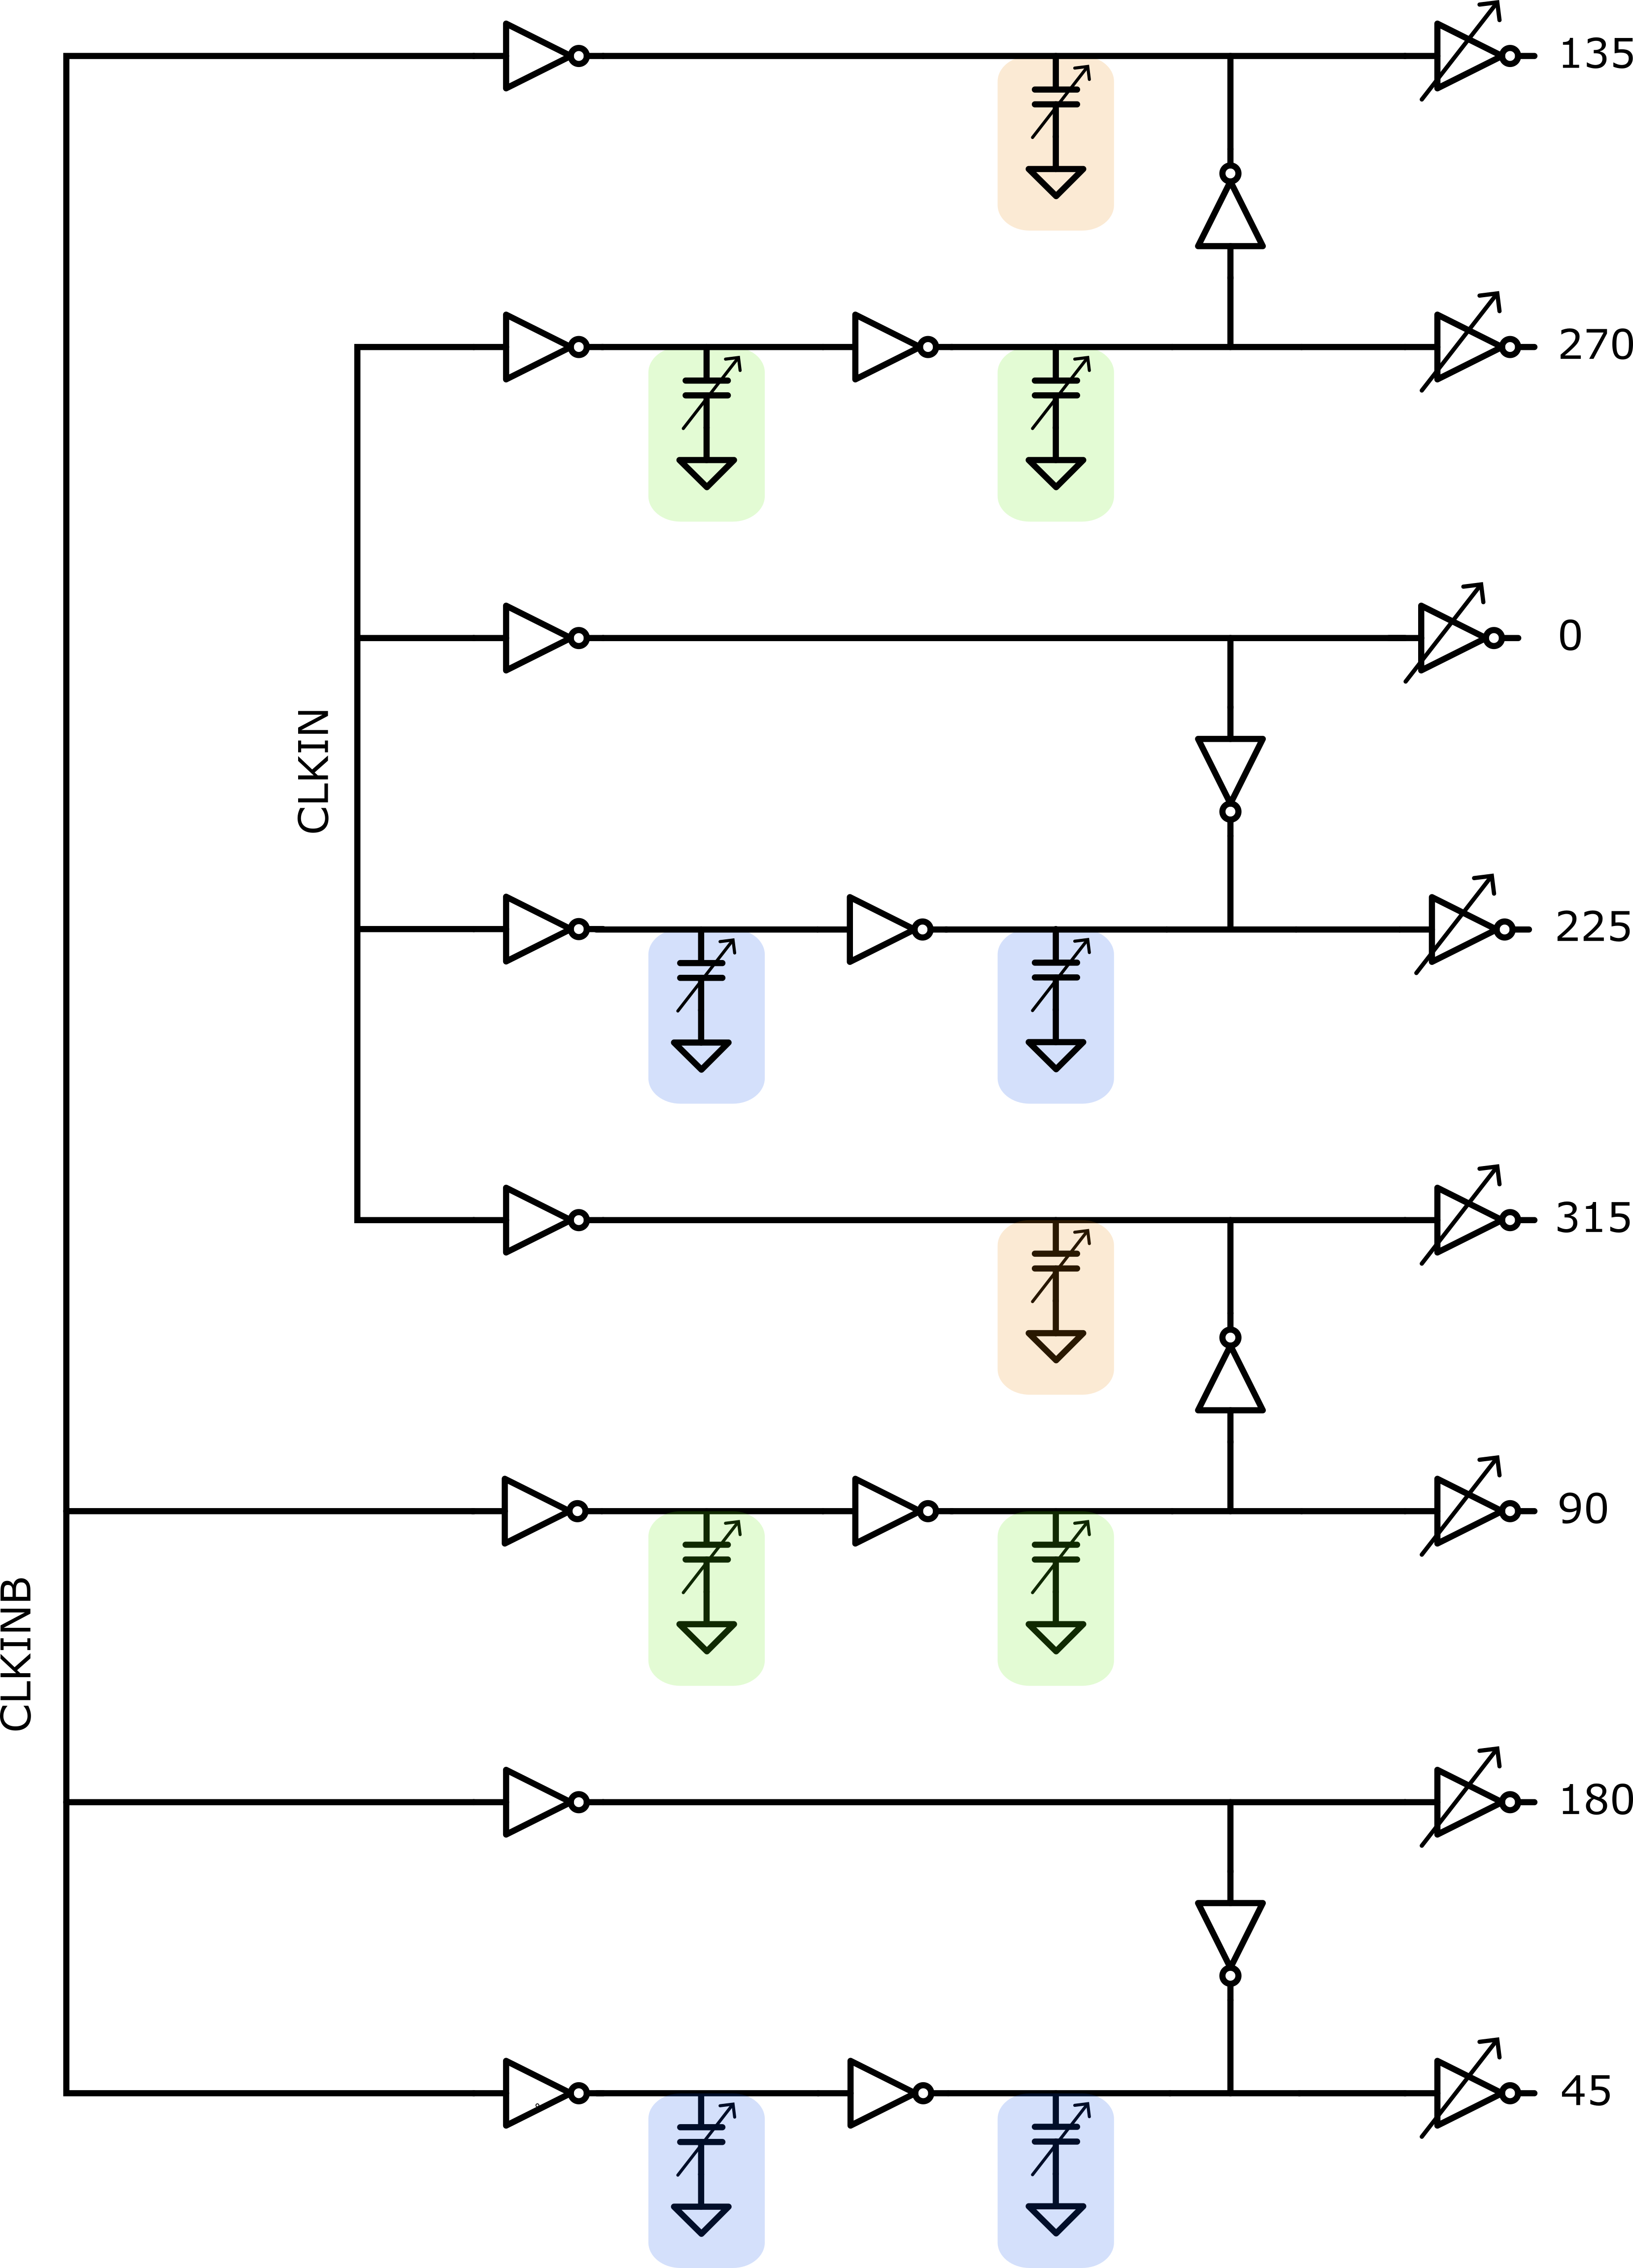
\includegraphics[width=0.6\linewidth]{figures/Schematics/ff_8out.png}
  \caption{Feed-forward phase interpolator with eight outputs. The \ang{135}/\ang{315} and \ang{45}/\ang{225} phases are generated by mixing the \ang{0}/\ang{180} and \ang{270}/\ang{90} phases into branches similar to those of \ang{0}/\ang{180} and \ang{270}/\ang{90} phases, respectively.}
  \label{fig:FF_8out}
\end{figure}

\begin{figure}[htbp]
  \hfill
  \begin{subfigure}[b]{0.1\linewidth}
    \centering
    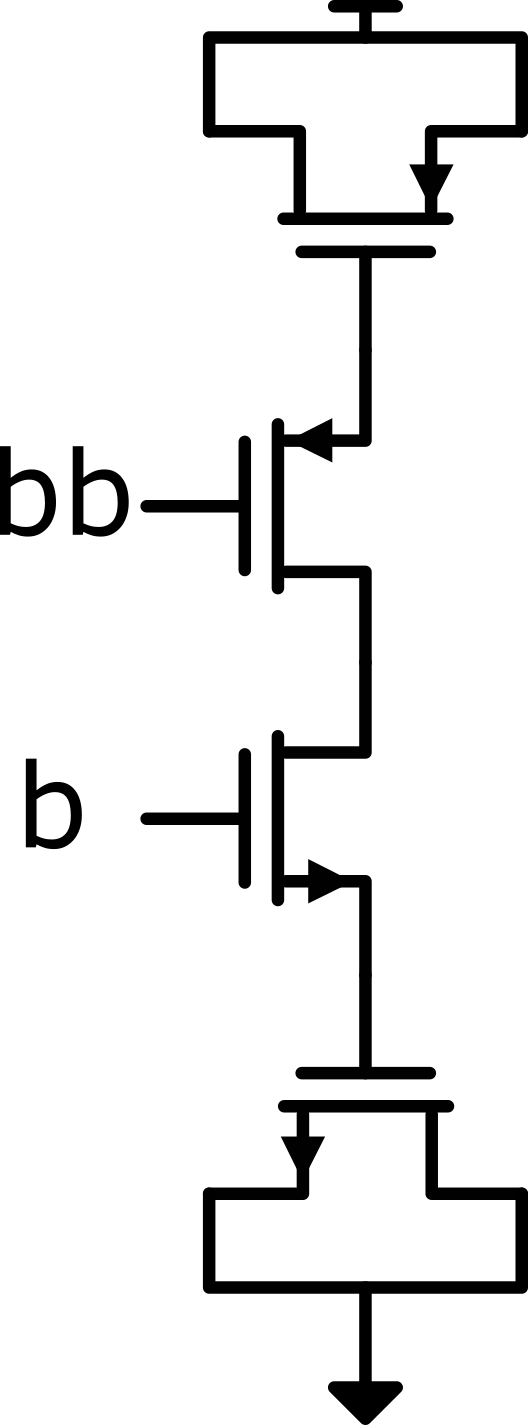
\includegraphics[width=\linewidth]{figures/Schematics/2P2N_cap.png}
    \caption{2P2N Capacitor Bank Unit Cell}
    \label{fig:2P2N_cap}
  \end{subfigure}
  \hfill
  \begin{subfigure}[b]{0.15\linewidth}
    \centering
    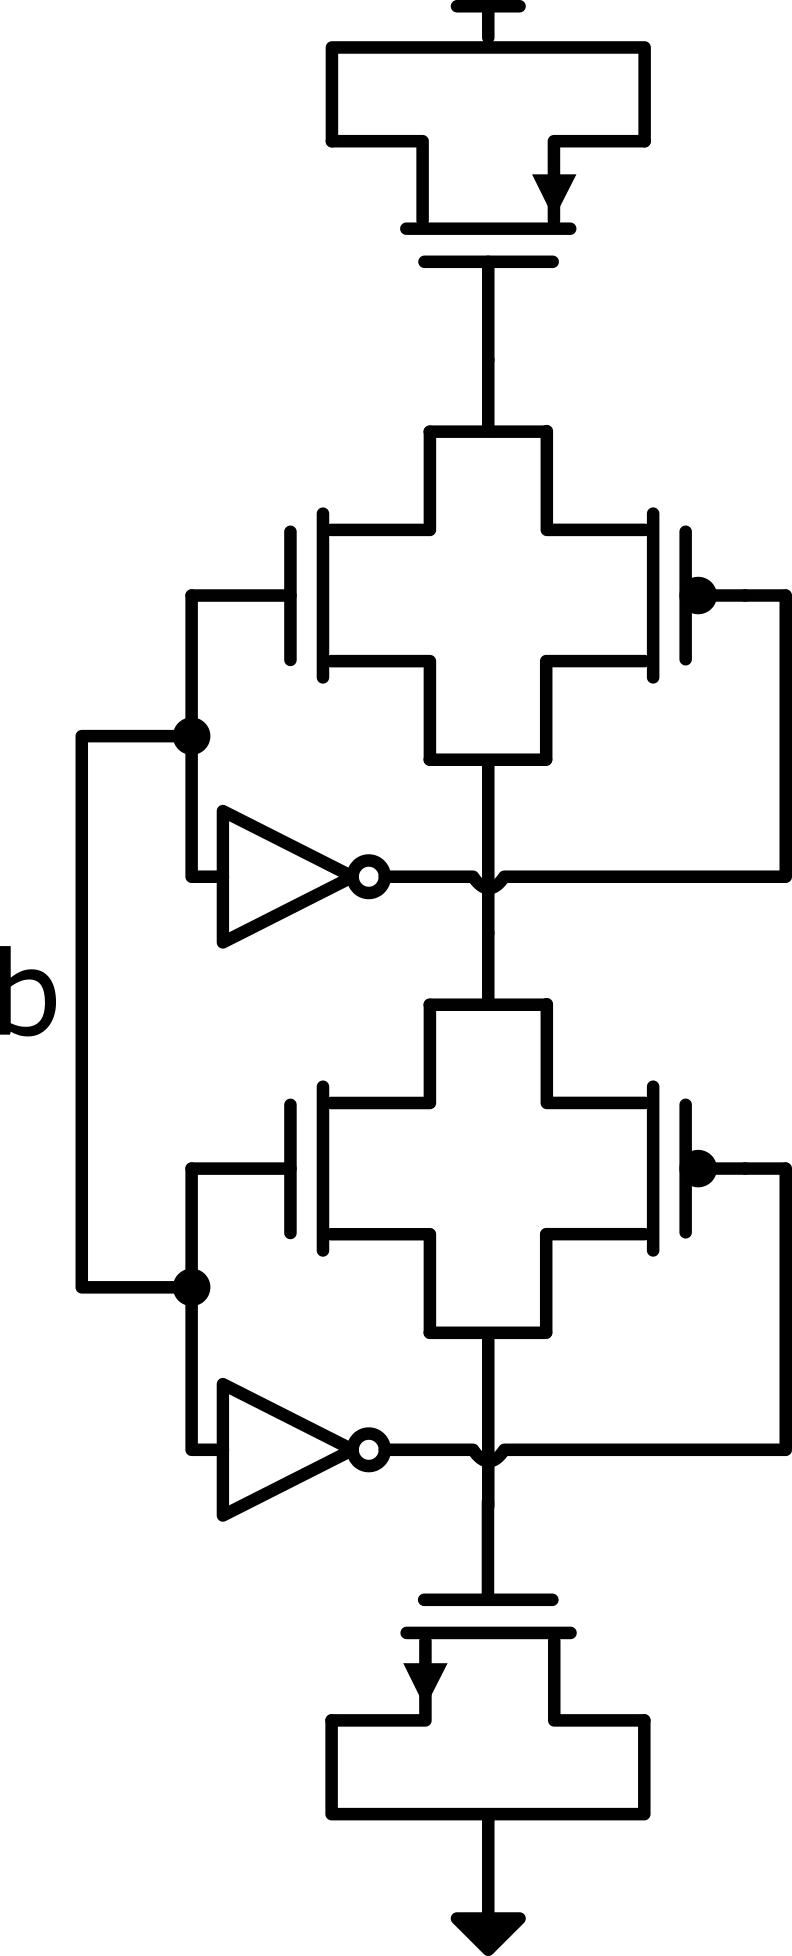
\includegraphics[width=\linewidth]{figures/Schematics/Tgate_cap.png}
    \caption{Tgate Capacitor Bank Unit Cell}
    \label{fig:Tgate_cap}
  \end{subfigure}
  \hfill
  \begin{subfigure}[b]{0.1\linewidth}
    \centering
    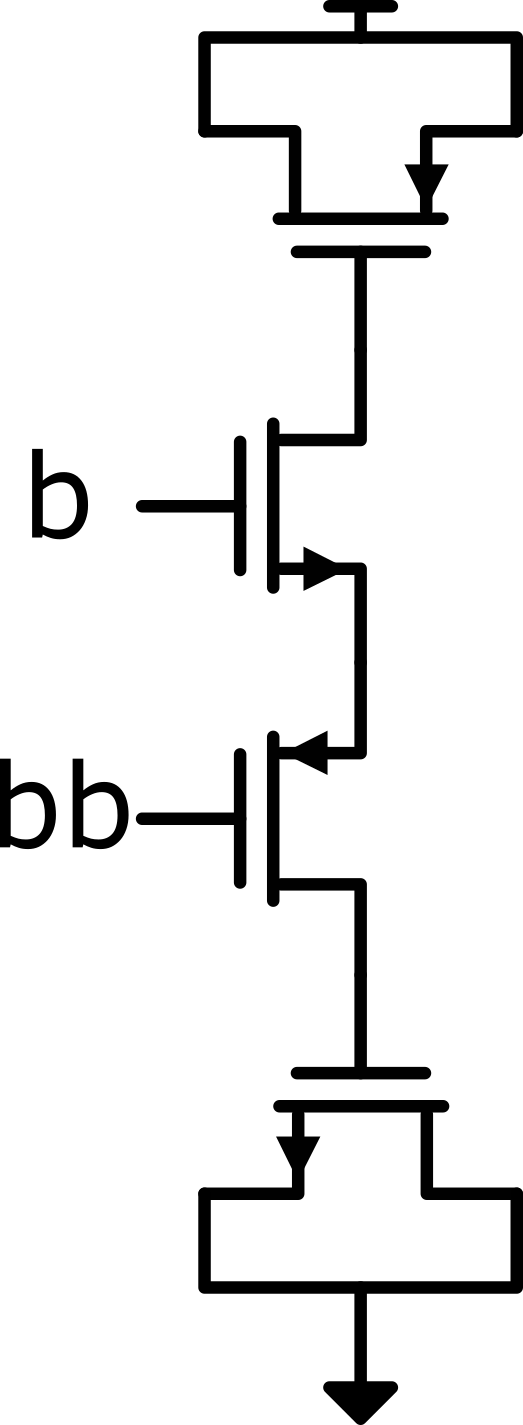
\includegraphics[width=\linewidth]{figures/Schematics/PNPN_cap.png}
    \caption{PNPN Capacitor Bank Unit Cell}
    \label{fig:PNPN_cap}
  \end{subfigure}
  \hfill\null
  \caption{Different capacitor bank implementations for the feed-forward phase interpolator.}
\end{figure}

\begin{figure}[htbp]
  \centering
  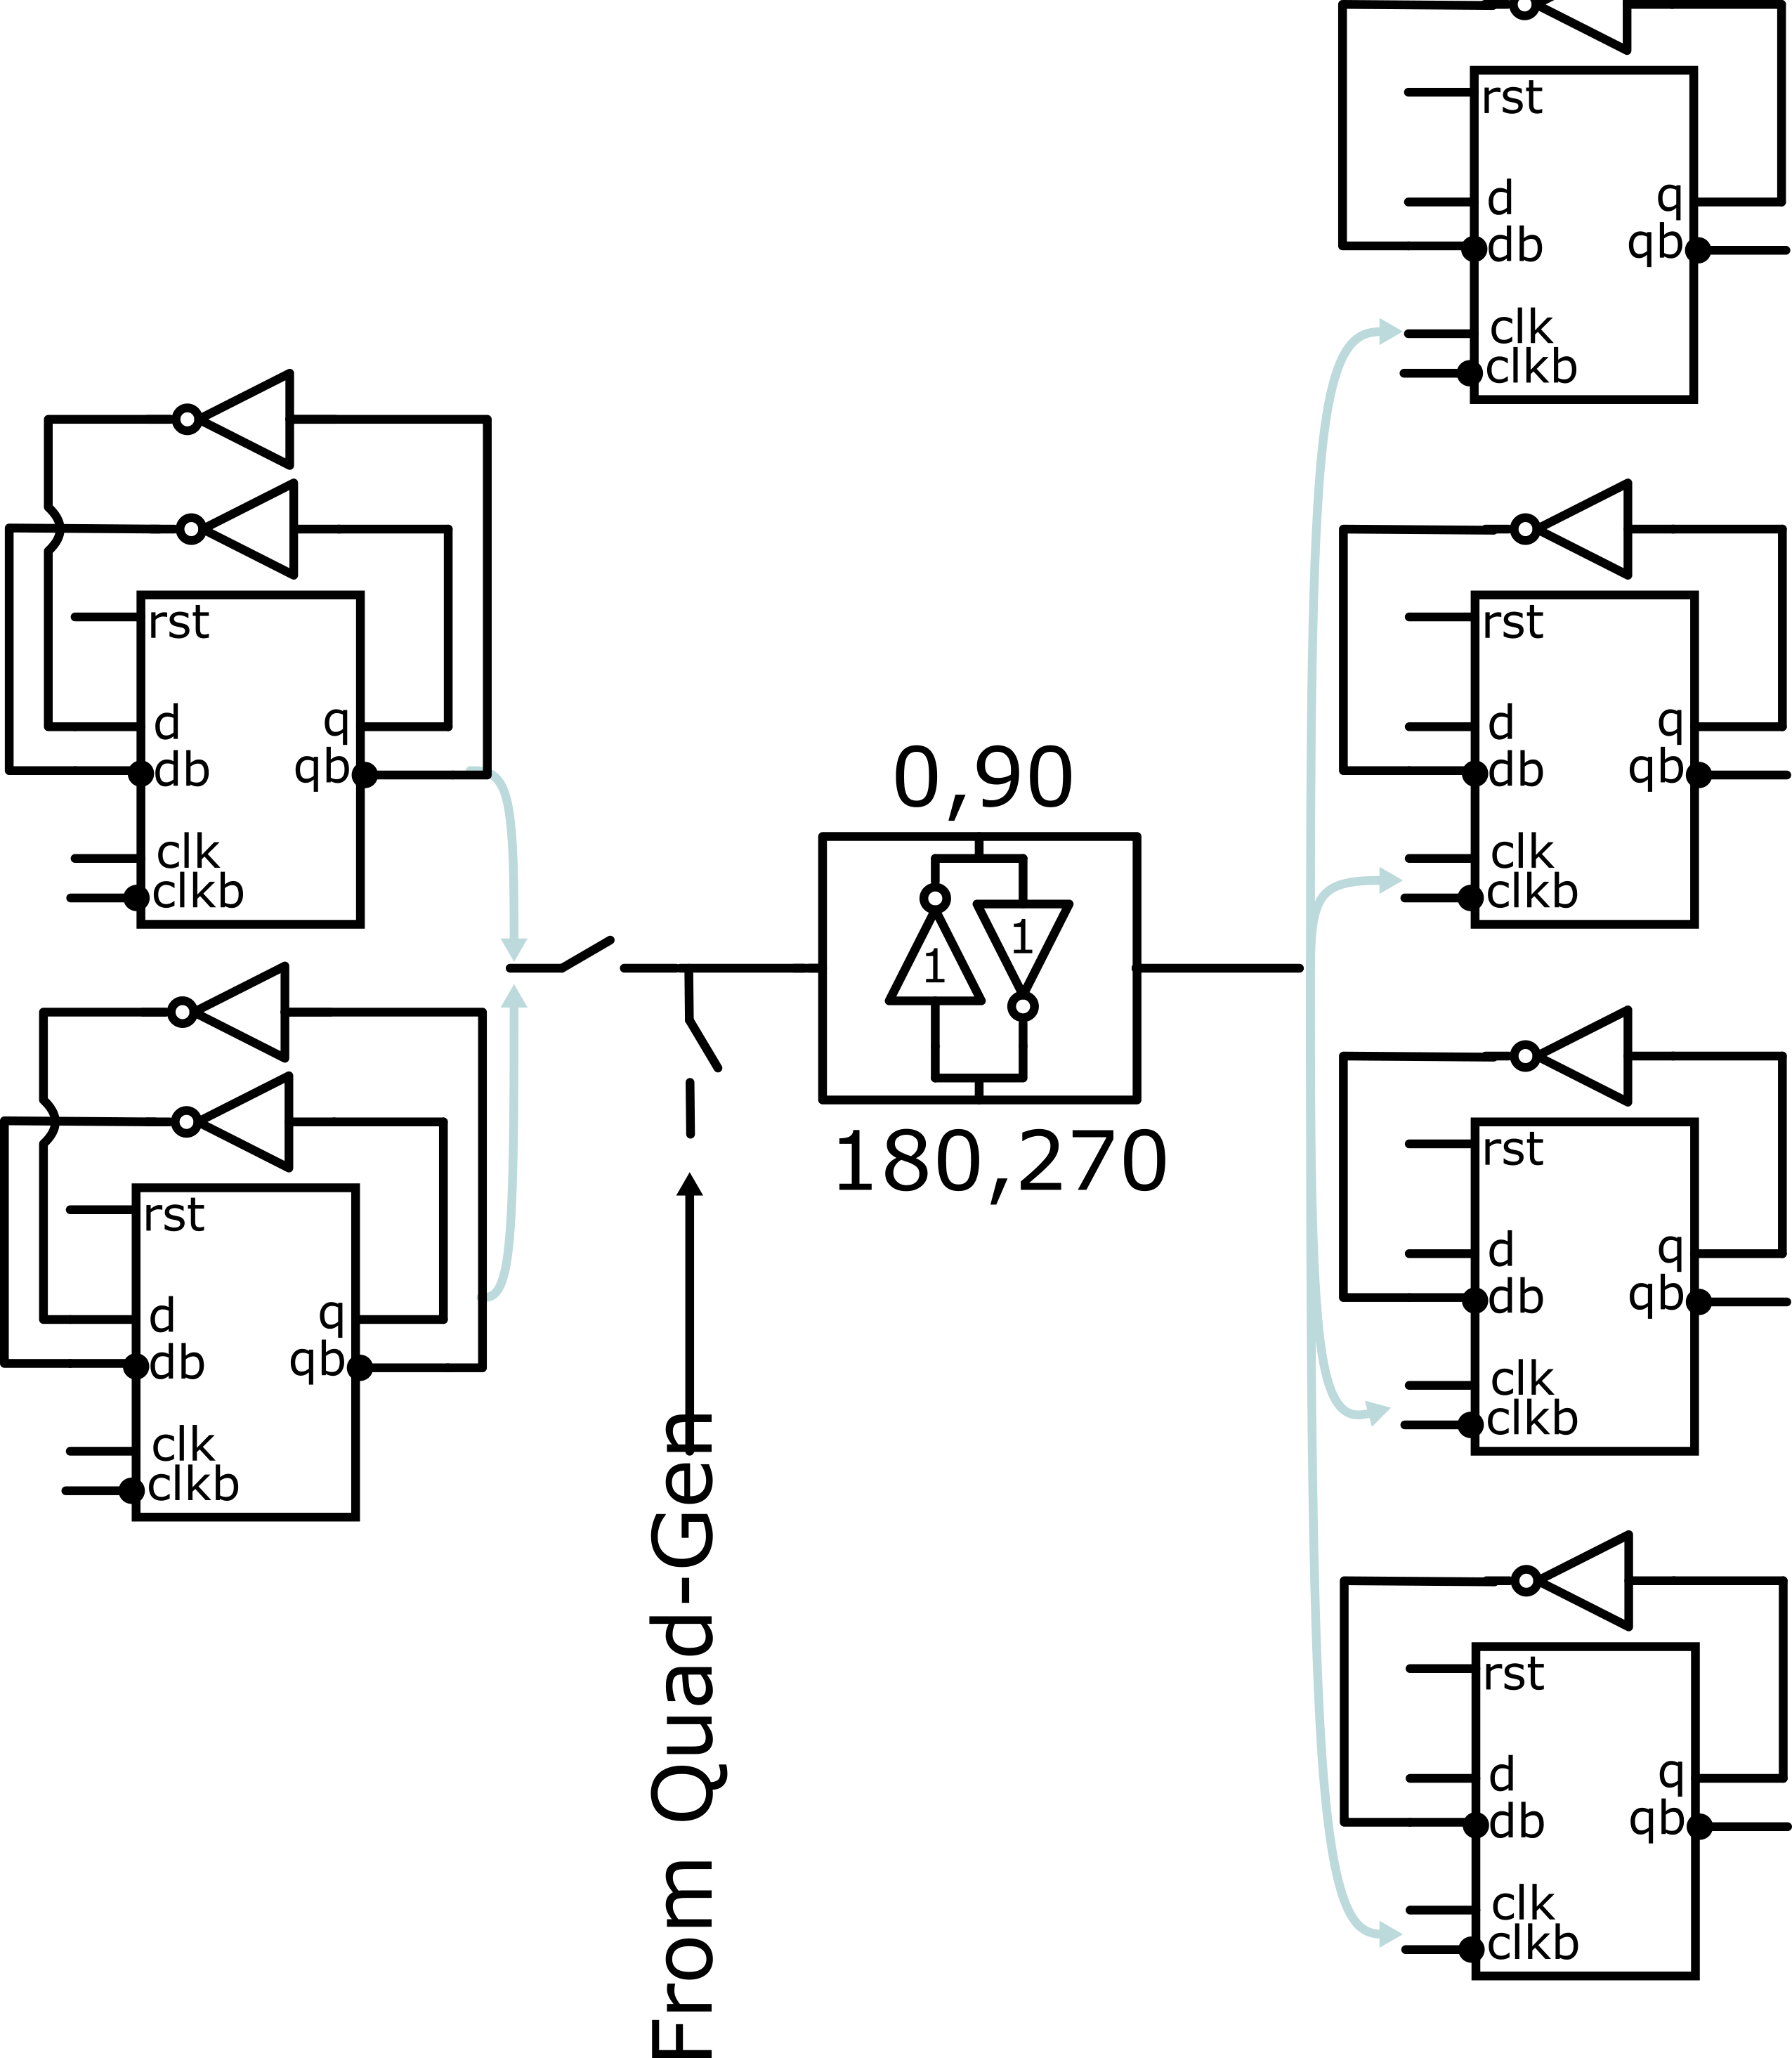
\includegraphics[width=0.5\linewidth]{figures/Schematics/2stage_divider.png}
  \caption{Schematic of the first implementation of the 2-stage clock divider. The first stage consists of two flip-flops, while the second stage consists of four flip-flops sampling the output clocks from the first stage.}
  \label{fig:2stage_divider}
\end{figure}

\begin{figure}[htbp]
  \centering
  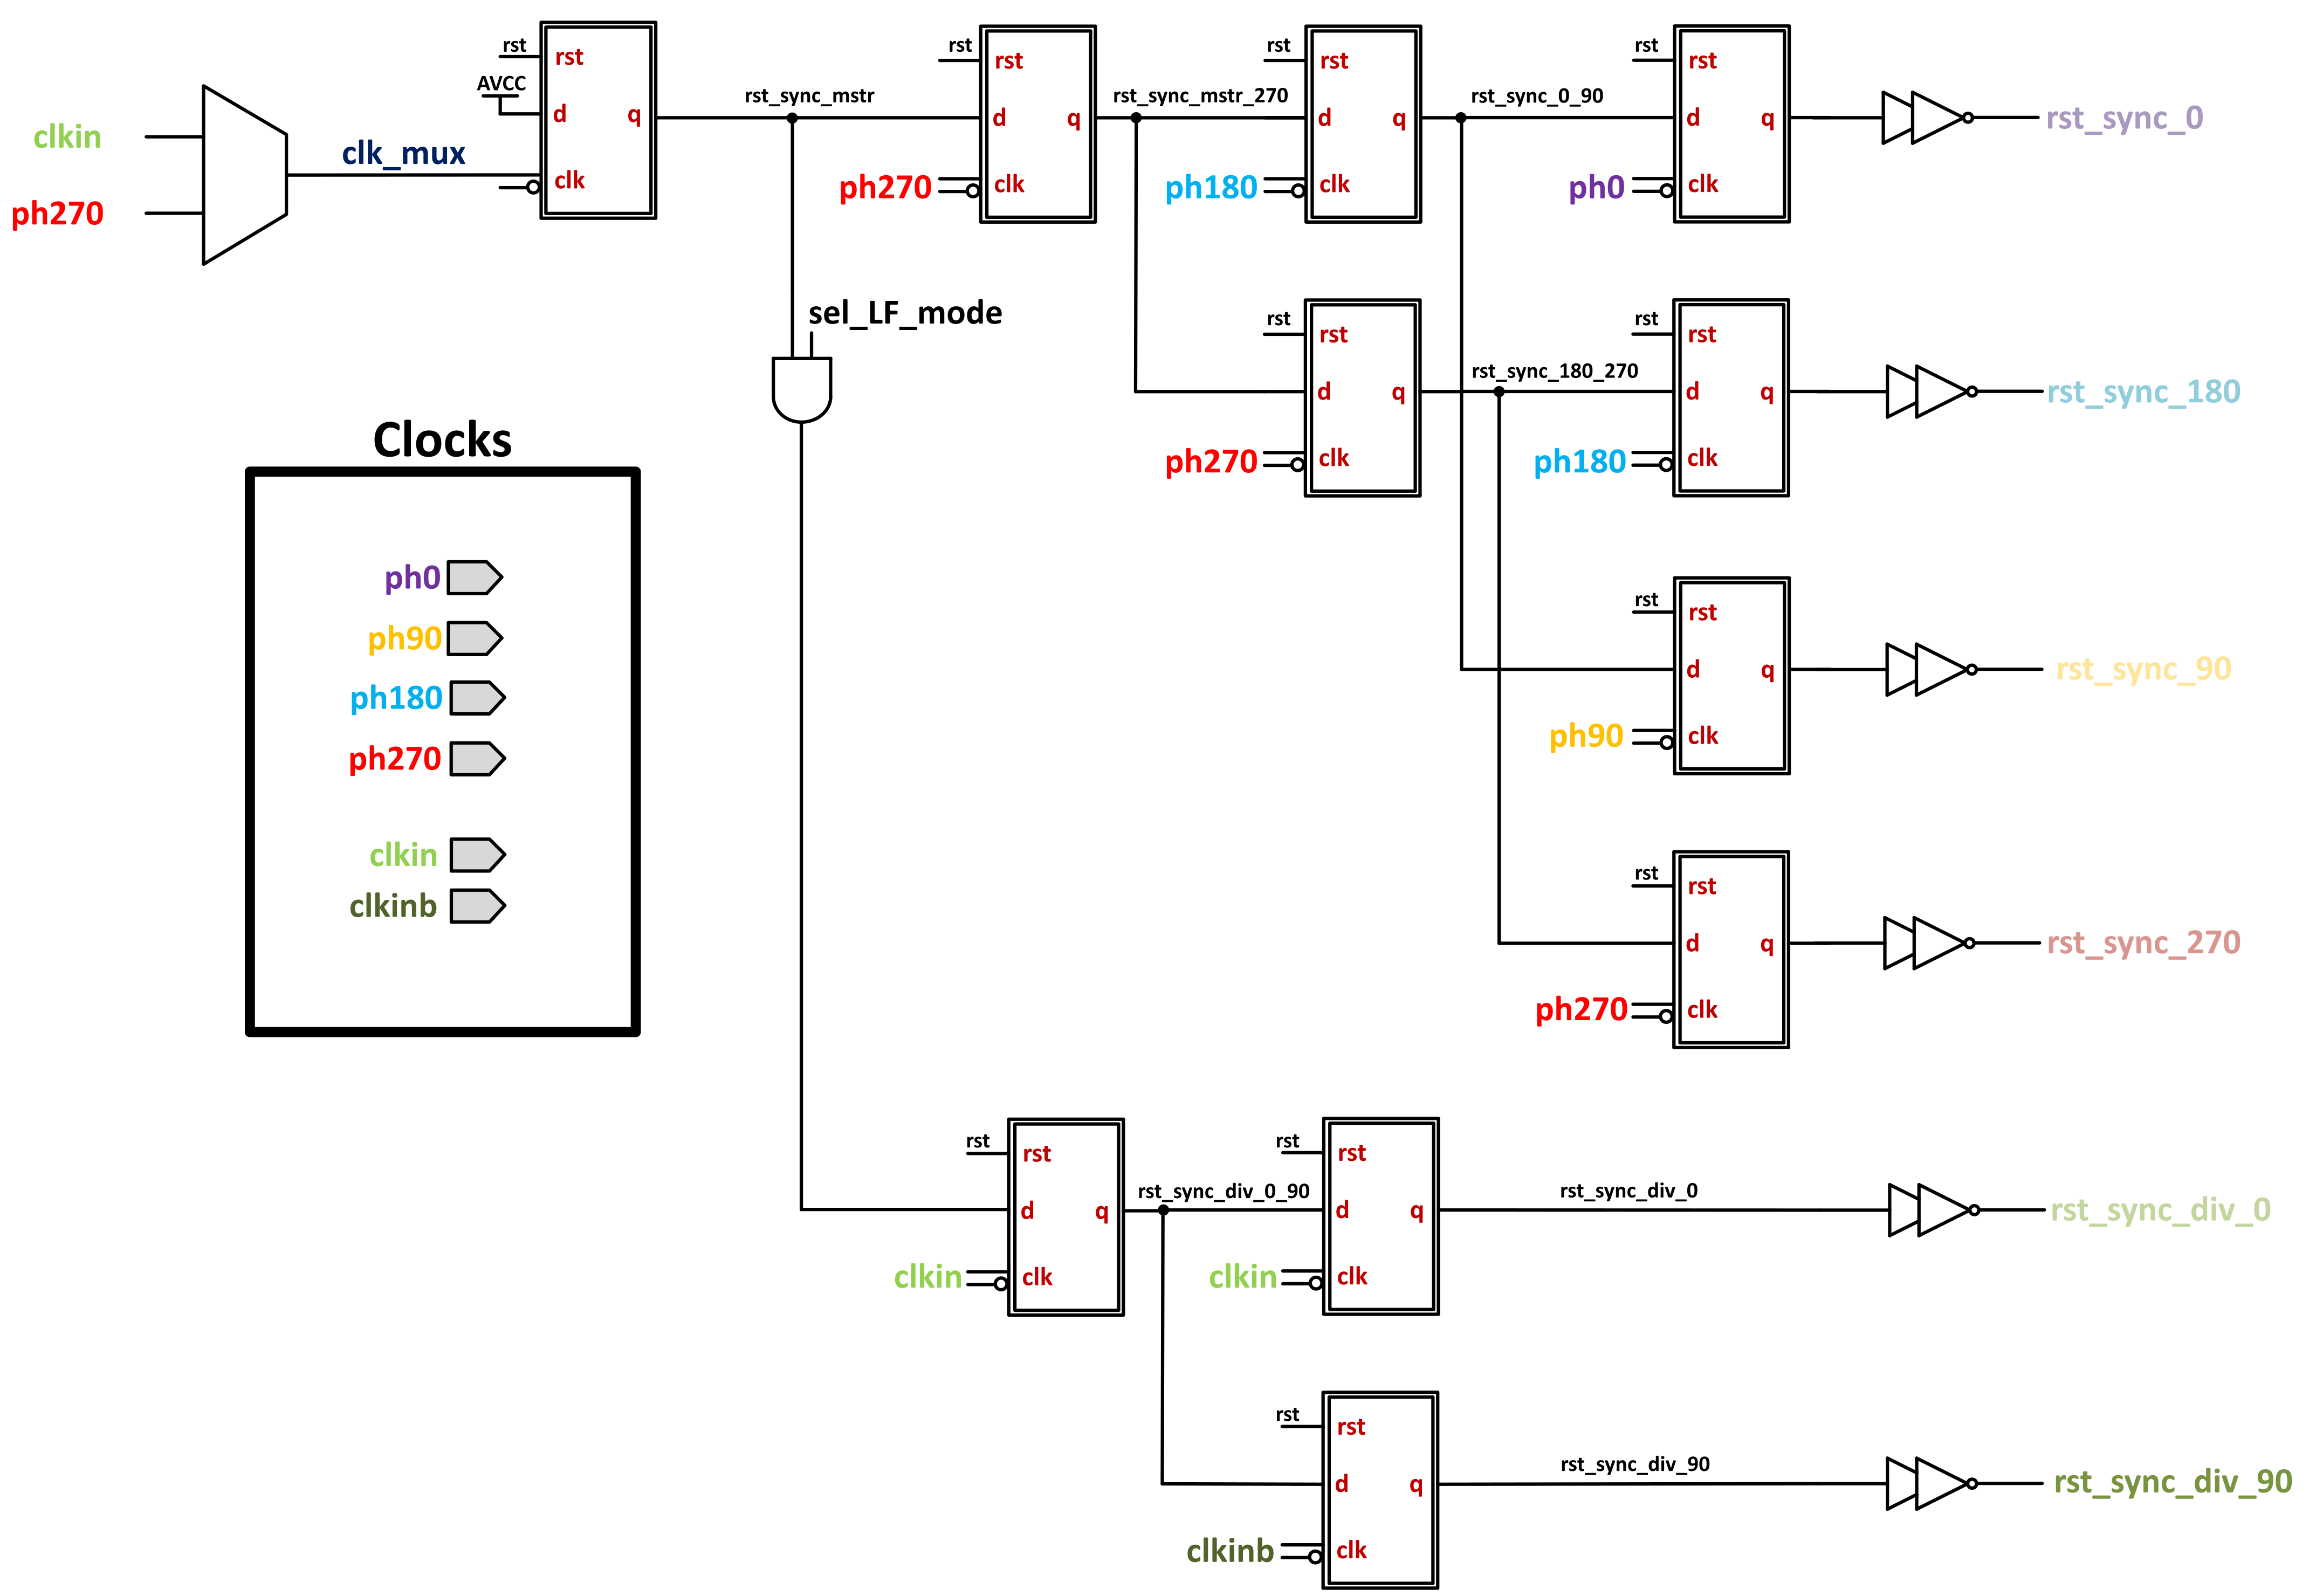
\includegraphics[width=\linewidth]{figures/Schematics/reset_seq.png}
  \caption{Reset sequence logic for the 2-stage clock divider. The reset is triggered by clock \ang{180} in LF mode and clock \ang{270} in MF mode, ensuring that consecutive flip-flops are clocked by clocks that are at least \ang{180} apart.}
  \label{fig:reset_seq}
\end{figure}